\documentclass[letter,12pt]{article}
\usepackage[paperheight=27.94cm,paperwidth=21.59cm,bindingoffset=0in,left=3cm,right=2.0cm, top=3.5cm,bottom=2.5cm, headheight=200pt, headsep=1.0\baselineskip]{geometry}
\usepackage{graphicx}
\usepackage{subcaption}
\usepackage[spanish]{babel}
\usepackage{xcolor}
\usepackage[utf8]{inputenc}
\usepackage{float}
\usepackage{hyperref}
\usepackage{listings}

% ---- Definicion minima de "json" como lenguaje para listings (no viene por defecto) ----
\lstdefinelanguage{json}{
  basicstyle=\ttfamily\footnotesize,
  showstringspaces=false,
  breaklines=true,
  keywords={true,false,null},
  keywordstyle=\bfseries,
  literate=
    *{0}{{{\color{black}0}}}{1}
     {1}{{{\color{black}1}}}{1}
     {2}{{{\color{black}2}}}{1}
     {3}{{{\color{black}3}}}{1}
     {4}{{{\color{black}4}}}{1}
     {5}{{{\color{black}5}}}{1}
     {6}{{{\color{black}6}}}{1}
     {7}{{{\color{black}7}}}{1}
     {8}{{{\color{black}8}}}{1}
     {9}{{{\color{black}9}}}{1},
}

% ---- Configuracion para bloques de codigo/JSON (evita que el texto se salga de la hoja) ----
\lstset{
  basicstyle=\ttfamily\footnotesize,
  breaklines=true,
  breakatwhitespace=false,
  columns=fullflexible,
  frame=single,
  backgroundcolor=\color{black!3},
  rulecolor=\color{black!40},
  showstringspaces=false,
  xleftmargin=2pt,
  xrightmargin=2pt
}

\setlength{\emergencystretch}{3em} % evita pequenos desbordes con texttt largos sin romper el diseno

% ---- Sangria: solo el primer parrafo de cada seccion/subseccion lleva sangria.
% Se desactiva la sangria automatica de todos los parrafos (asi el texto que
% viene despues de un recuadro de codigo, figura o lista ya no aparece
% desplazado a la derecha) y se agrega un pequeno espacio entre parrafos para
% que sigan distinguiendose unos de otros sin necesidad de sangria.
\setlength{\parindent}{0pt}
\setlength{\parskip}{0.55\baselineskip plus 0.1\baselineskip minus 0.1\baselineskip}
\newcommand{\sangria}{\hspace*{1.25cm}} % usar al inicio del primer parrafo de cada seccion

% ---- Carpeta donde estan todas las figuras ----
\graphicspath{{figuras/}}

\begin{document}

% ---- Nombres de elementos flotantes forzados a español ----
% (se fuerzan explícitamente porque, dependiendo del motor/instalación de
% babel usada para compilar, el paquete puede no cargar el idioma español
% y recurrir por defecto a los nombres en inglés "Figure"/"Table"/"Contents";
% esto evita que las figuras del documento final queden rotuladas en inglés).
\renewcommand{\figurename}{Figura}
\renewcommand{\contentsname}{Índice}
\renewcommand{\tablename}{Tabla}

\shorthandoff{"} % evita que "u, "a, etc. se interpreten como ü, ä (atajos de babel-spanish) dentro de \texttt{...}

   \title{\Huge{Informe Laboratorio 3}}

   \author{\textbf{Sección 2} \\  \\ Francisco Polanco \\ e-mail: francisco.polanco@mail.udp.cl}

   \date{Octubre de 2026}

   \maketitle

   \tableofcontents

  \newpage


\section{Descripción de actividades}
\label{sec:enunciado}
\sangria El laboratorio tiene como propósito examinar cómo una aplicación web procesa las contraseñas desde el navegador, identificar los mecanismos criptográficos utilizados durante el registro y el inicio de sesión, y evaluar si un valor de autenticación derivado puede reutilizarse sin introducir la contraseña original. Para ello, se analizó el intercambio de solicitudes entre el cliente y el servidor, se reprodujo el cálculo criptográfico desde la consola y se realizó una prueba controlada de modificación de tráfico sobre una cuenta creada exclusivamente para la actividad.\par

Como medida de seguridad, la contraseña utilizada en las pruebas debía reemplazarse al finalizar las actividades, de modo que los valores capturados durante el laboratorio dejaran de corresponder a la credencial vigente.\par

El desarrollo se organizó según los criterios solicitados en la rúbrica:

\begin{itemize}
    \item Identificación del algoritmo de hash utilizado para las contraseñas al momento del registro en el sitio.

    \item Identificación del algoritmo de hash utilizado para las contraseñas al momento de iniciar sesión.

    \item Generación del hash de la contraseña desde la consola del navegador, partiendo de la contraseña en texto plano.

    \item Interceptación del tráfico de login utilizando BurpSuite desde su equipo.

    \item Realización de un intento de login, modificando una contraseña incorrecta por el hash obtenido en el punto anterior.

    \item Descripción de las políticas de privacidad o seguridad relacionadas con las contraseñas, incluyendo un enlace a las mismas.

    \item Cuatro conclusiones sobre la seguridad o vulnerabilidad de la implementación observada.

\end{itemize}

\section{Desarrollo de actividades según criterio de rúbrica}

\subsection{Identifica el algoritmo de hash utilizado al momento de registrarse en el sitio}
\label{sec:registro}

\sangria Se seleccionó \textbf{Mega} (\url{https://mega.nz}) y se creó una cuenta de prueba destinada únicamente al laboratorio. Antes de ingresar los datos del formulario, se abrieron las herramientas de desarrollador del navegador y se accedió a la pestaña \textit{Network}. Se aplicó el filtro \textit{XHR} para concentrar la revisión en las solicitudes de la aplicación y se habilitó \textit{Preserve log} para conservar los registros durante los cambios de página. Con esta preparación fue posible observar el proceso completo de registro y distinguir las solicitudes dirigidas a la API \texttt{https://g.api.mega.co.nz/cs}.

El registro no se resolvió mediante una única petición: el navegador intercambió varias solicitudes \texttt{POST} con distintas acciones identificadas por el campo \texttt{a}. Se revisaron sus cuerpos JSON y se relacionaron con las etapas visibles del formulario, la verificación del correo y la configuración inicial de la cuenta. Esta revisión permitió separar los datos de perfil de los valores utilizados en la preparación de claves y la autenticación. Los mensajes más relevantes fueron los siguientes:


\begin{itemize}
\item \textbf{Paquete 1 — creación de la cuenta}: en todas las solicitudes a la API de Mega, el campo \texttt{a} ("acción") indica qué operación está pidiendo el cliente al servidor. En la Figura~\ref{fig:registro-up-kts} se observa esta solicitud capturada directamente desde la pestaña \textit{Network} del navegador durante el formulario de registro.

    \begin{figure}[H]
        \centering
        \begin{subfigure}[b]{\textwidth}
            \centering
            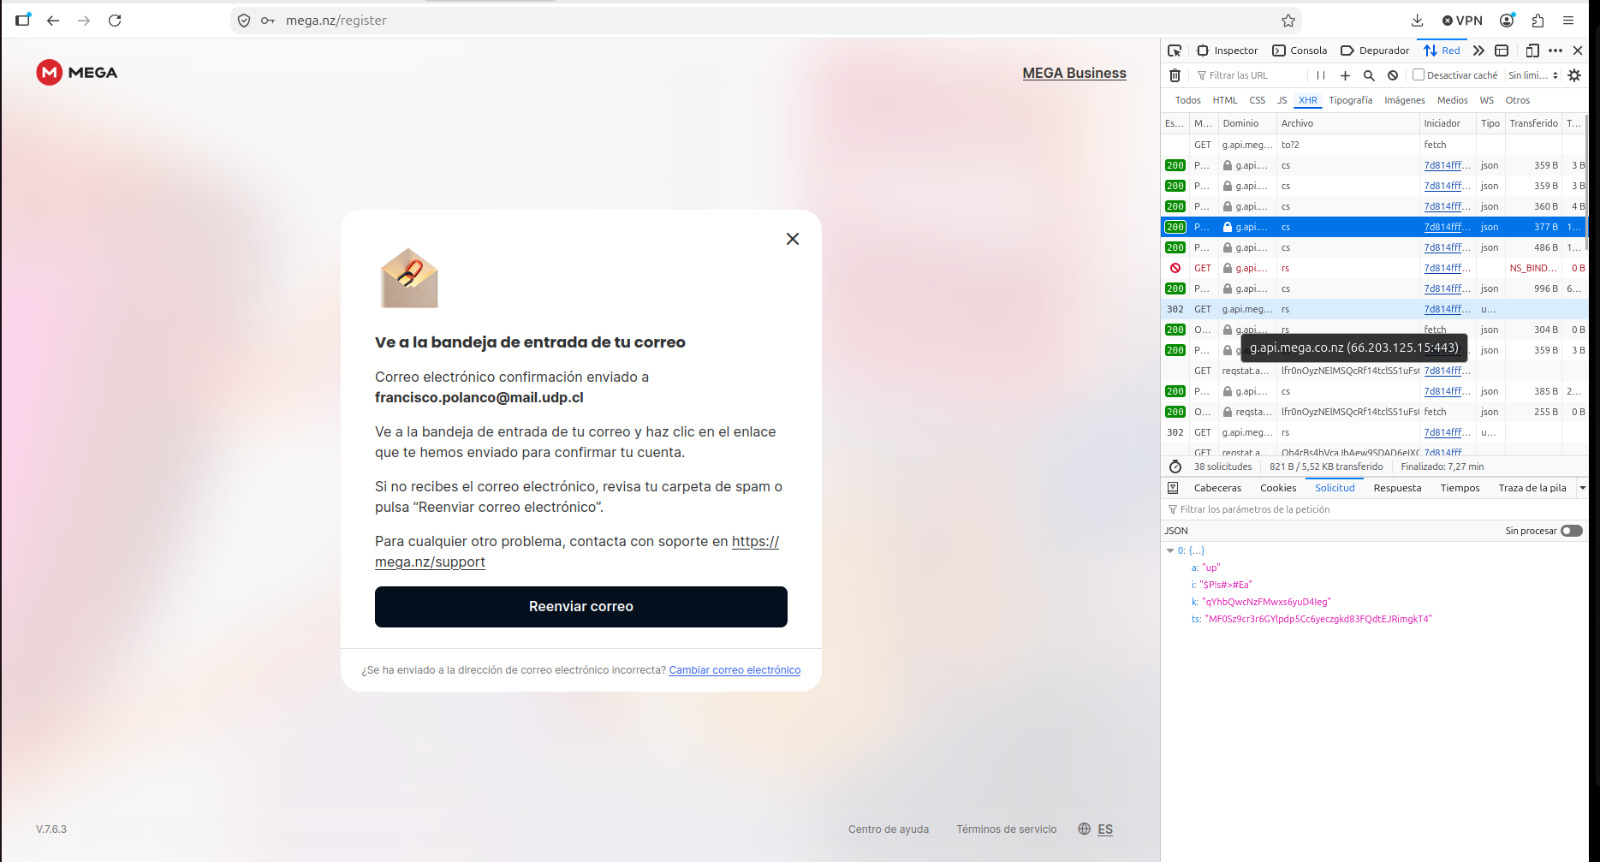
\includegraphics[width=0.85\textwidth]{fig01_registro_up_k_ts_orig.jpeg}
            \caption{Captura original.}
        \end{subfigure}
        \vspace{0.4cm}
        \begin{subfigure}[b]{\textwidth}
            \centering
            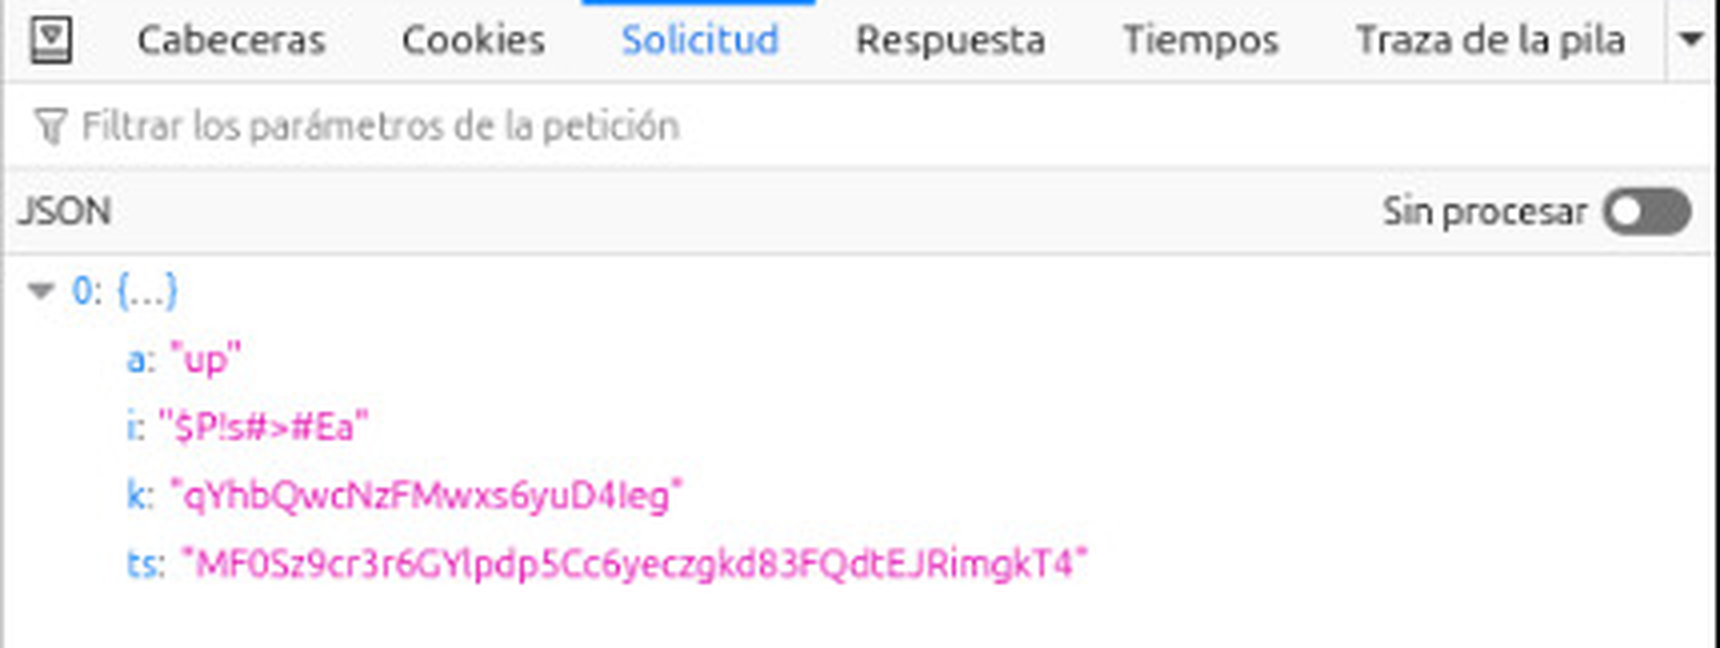
\includegraphics[width=0.85\textwidth]{fig01_registro_up_k_ts_recorte.png}
            \caption{Recorte ampliado para mayor legibilidad.}
        \end{subfigure}
        \caption{Solicitud de creación de cuenta (\texttt{a: "up"}) capturada en la pestaña \textit{Network}, mostrando los campos \texttt{k} (master key cifrada) y \texttt{ts} (desafío de verificación).}
        \label{fig:registro-up-kts}
    \end{figure}

    El cuerpo JSON de esta solicitud, tal como aparece en la figura anterior, es el siguiente:
\begin{lstlisting}[language=json]
{
  "a": "up",
  "i": "$P!s#>#Ea",
  "k": "qYhbQwcNzFMwxs6yuD4Ieg",
  "ts": "MF0Sz9cr3r6GYlpdp5Cc6yeczgkd83FQdtEJRimgkT4"
}
\end{lstlisting}

    A continuación se detalla el objetivo de cada campo del mensaje:

    \begin{itemize}
        \item \texttt{a}: tiene el valor \texttt{"up"} (\textit{update user}), la acción que Mega usa tanto para crear el perfil inicial de una cuenta como para modificarlo más adelante; es el campo que le dice al servidor qué tipo de operación debe ejecutar con el resto de los datos del mensaje.

        \item \texttt{i}: es un identificador de relación generado por el cliente (una cadena aleatoria corta) que acompaña a la solicitud únicamente para que el navegador pueda emparejar la respuesta del servidor con la petición que la originó, de forma similar a un id. No tiene ninguna función criptográfica.

        \item \texttt{k}: contiene la \textit{master key} de la cuenta cifrada. Mega genera, para cada cuenta nueva, una clave simétrica aleatoria de 128 bits llamada \textit{master key}, que es la que realmente se usa para cifrar y descifrar todos los archivos y demás claves de usuarios. Como esta clave no puede viajar ni almacenarse en texto plano, antes de enviarla al servidor el navegador la cifra usando \textbf{AES} (\textit{Advanced Encryption Standard}), un algoritmo de cifrado simétrico por bloques que es el estándar actual para este tipo de operaciones. La clave usada para este cifrado AES no es la contraseña en sí, sino una clave derivada de ella. 

        \item \texttt{ts}: es un valor de desafío (\textit{challenge}) que el cliente genera para que el servidor pueda, en inicios de sesión futuros, confirmar que quien se conecta es capaz de reconstruir correctamente la \textit{master key} a partir de la contraseña, sin que la contraseña ni un hash directo de ella tengan que viajar por la red. 
    \end{itemize}


 \item \textbf{Paquete 2 — datos de perfil (\texttt{a: "up"})}: después de que el Paquete 1 establece la \textit{master key} cifrada de la cuenta, el navegador envía una segunda solicitud, también con la acción \texttt{up}, para completar el perfil del usuario (nombre y aceptación de términos) y así poder avanzar al siguiente paso del flujo de registro: la confirmación de la cuenta, capturada justo a continuación en el Paquete 3. La Figura~\ref{fig:registro-confirmacion} muestra, en su primera subfigura, la pantalla de confirmación que Mega despliega inmediatamente después de enviar este paquete, y en la segunda subfigura, la solicitud correspondiente capturada en el panel de \textit{Network}.

    \begin{figure}[H]
        \centering
        \begin{subfigure}[b]{\textwidth}
            \centering
            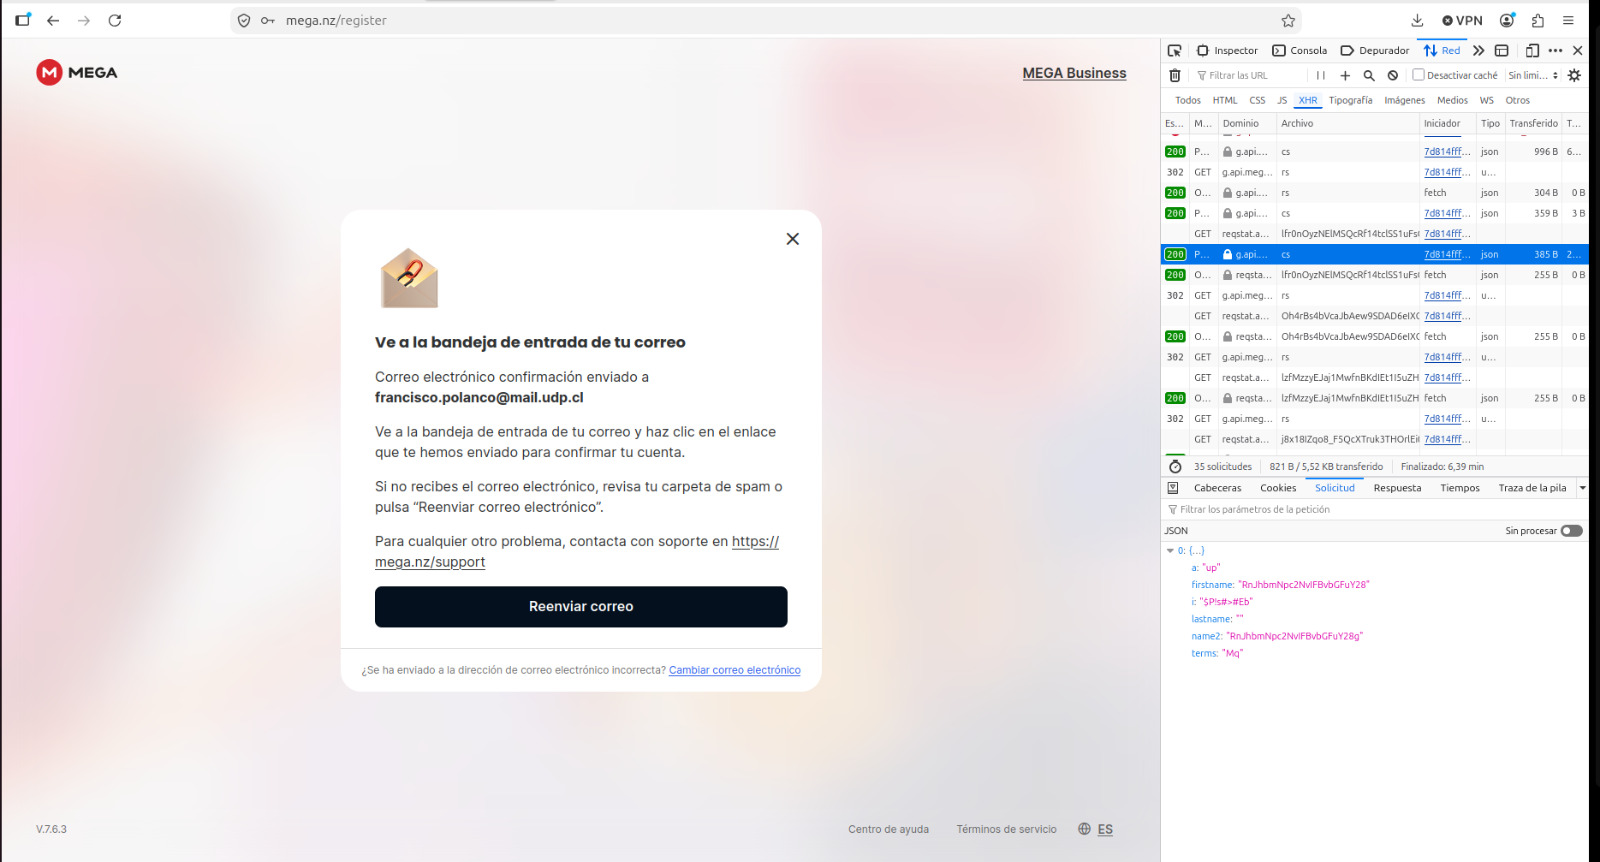
\includegraphics[width=0.85\textwidth]{fig02_registro_confirmacion_up_perfil_orig.jpeg}
            \caption{Captura original.}
        \end{subfigure}
        \vspace{0.4cm}
        \begin{subfigure}[b]{\textwidth}
            \centering
            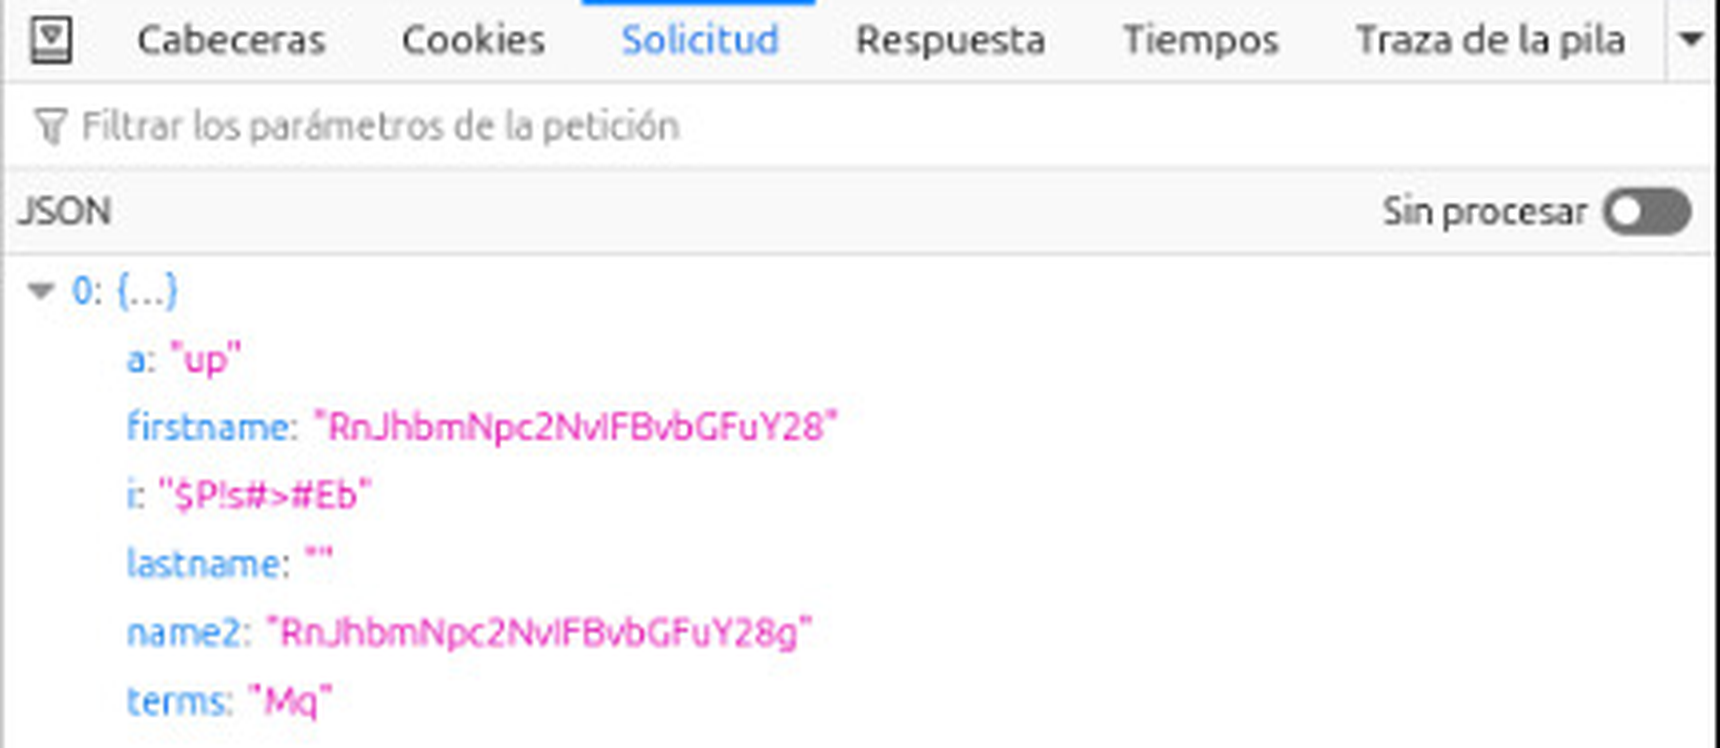
\includegraphics[width=0.85\textwidth]{fig02_registro_confirmacion_up_perfil_recorte.png}
            \caption{Recorte ampliado para mayor legibilidad.}
        \end{subfigure}
        \caption{Pantalla de confirmación de registro y solicitud \texttt{a: "up"} con los datos de perfil (\texttt{firstname}, \texttt{name2}, \texttt{terms}) codificados en Base64.}
        \label{fig:registro-confirmacion}
    \end{figure}

    El cuerpo JSON de la solicitud mostrada en la figura es el siguiente:
\begin{lstlisting}[language=json]
{
  "a": "up",
  "i": "$P)=FA<r",
  "firstname": "RnJhbmNpc2NvIFBvbGFuY28",
  "lastname": "",
  "name2": "RnJhbmNpc2NvIFBvbGFuY28g",
  "terms": "Mq"
}
\end{lstlisting}

    Los campos \texttt{firstname} y \texttt{name2} corresponden al nombre ingresado en el formulario, codificado en Base64  y \texttt{terms} registra la aceptación de los términos del servicio. Este paquete completa los datos del perfil, pero por sí solo todavía no confirma la cuenta ante el servidor: esa confirmación llega con la solicitud del Paquete 3, inmediatamente después de que el usuario valida el enlace enviado a su correo.

\item \textbf{Paquete 3 — confirmación de cuenta (\texttt{a: "uc2"})}: tras validar el enlace de confirmación recibido por correo electrónico, el navegador envía esta solicitud para cerrar formalmente el proceso de registro iniciado por los Paquetes 1 y 2. Es en este paquete donde aparece el campo que resuelve directamente el objetivo de esta sección: identificar qué algoritmo de hash usa Mega para proteger la contraseña al momento del registro. La Figura~\ref{fig:registro-uc2} muestra esta solicitud capturada en el navegador justo después de validar dicho enlace:

    \begin{figure}[H]
        \centering
        \begin{subfigure}[b]{\textwidth}
            \centering
            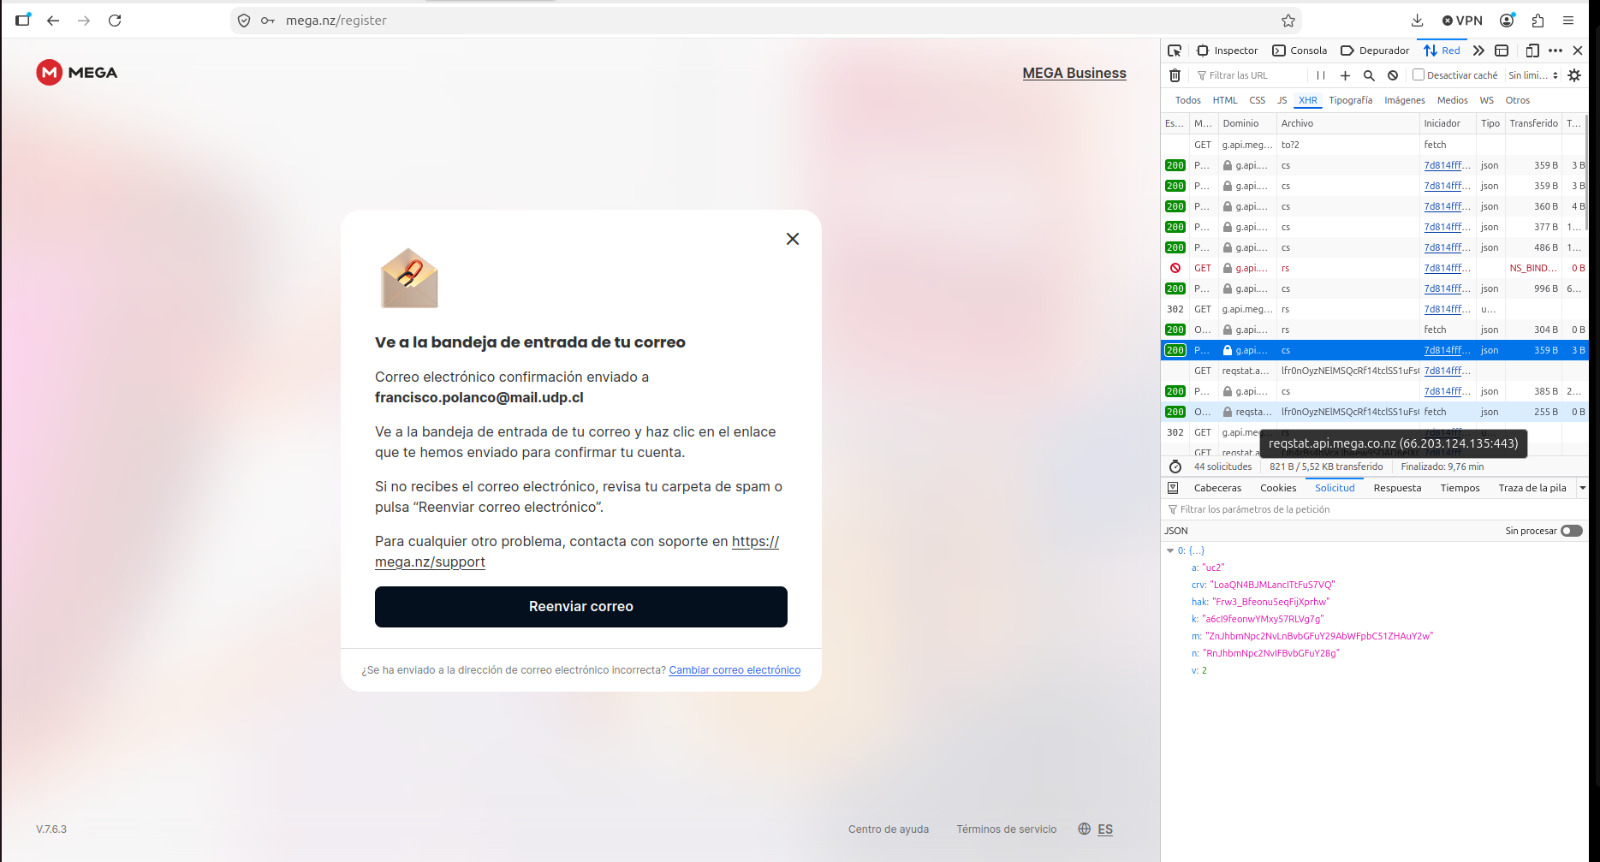
\includegraphics[width=0.85\textwidth]{fig03_registro_uc2_orig.jpeg}
            \caption{Captura original.}
        \end{subfigure}
        \vspace{0.4cm}
        \begin{subfigure}[b]{\textwidth}
            \centering
            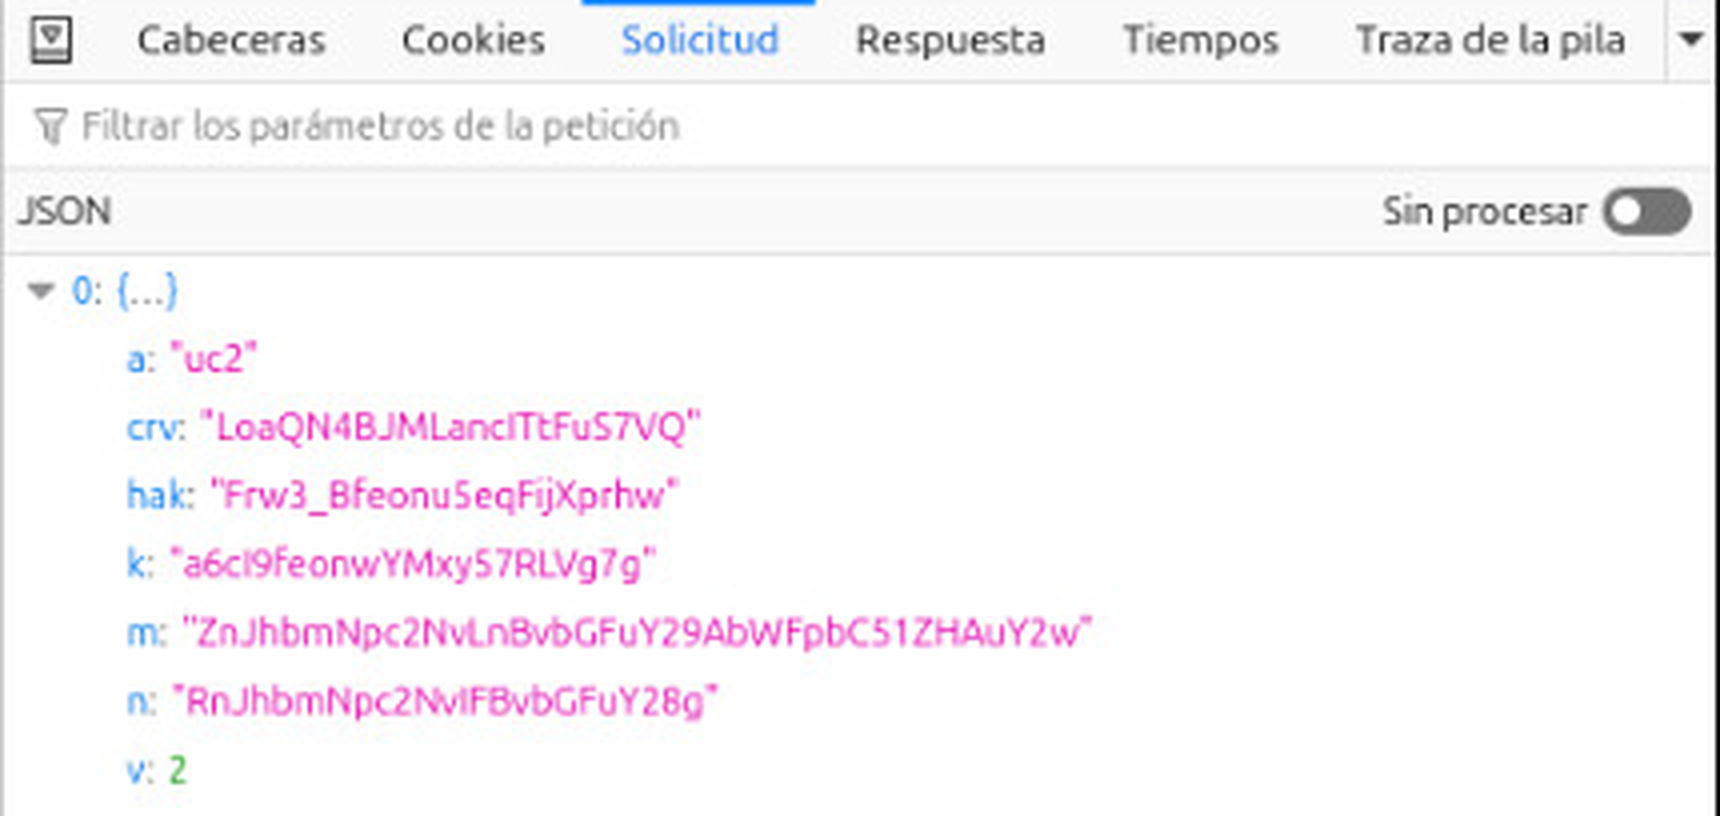
\includegraphics[width=0.85\textwidth]{fig03_registro_uc2_recorte.png}
            \caption{Recorte ampliado para mayor legibilidad.}
        \end{subfigure}
        \caption{Solicitud de confirmación de cuenta (\texttt{a: "uc2"}) tras validar el enlace enviado por correo, con el indicador \texttt{v: 2} del esquema de cuentas.}
        \label{fig:registro-uc2}
    \end{figure}

    El cuerpo JSON correspondiente a la solicitud de la figura anterior es el siguiente:
\begin{lstlisting}[language=json]
{
  "a": "uc2",
  "crv": "LoaQN4BJMLancITtFuS7VQ",
  "hak": "Frw3_Bfeonu5eqFijXprhw",
  "k": "a6cI9feonuYMxyS7RLVg7g",
  "m": "ZnJhbmNpc2NvLnBvbGFuY29AbWFpbC51ZHAuY2w",
  "n": "RnJhbmNpc2NvIFBvbGFuY28g",
  "v": 2
}
\end{lstlisting}

    Los campos \texttt{m} y \texttt{n} son el correo electrónico y el nombre del usuario codificados en Base64; \texttt{crv} y \texttt{k} son material cifrado de la cuenta (clave de verificación y \textit{master key}); y \texttt{hak} (\textit{hashed authentication key}) es un valor que el servidor guarda para comprobar, en el futuro, que el cliente conoce la \textit{password key} correcta, sin tener que almacenar esa clave ni la contraseña.

    El campo que realmente interesa para esta sección es \texttt{v}, con valor \textbf{2}. Este número no es un detalle menor del formato del mensaje: es el identificador del esquema de cuentas bajo el cual Mega procesa la contraseña de ese usuario, y Mega mantiene en paralelo dos esquemas distintos:

    \begin{itemize}
        \item \textbf{Esquema v1 (cuentas antiguas)}: la contraseña se procesa con un algoritmo propietario de Mega, no un estándar de la industria, que aplica 65.536 rondas sucesivas de cifrado AES en modo ECB sobre la contraseña para obtener el valor de autenticación.
        \item \textbf{Esquema v2 (cuentas nuevas)}: la contraseña se procesa mediante PBKDF2 (\textit{Password-Based Key Derivation Function 2}), un algoritmo estándar diseñado específicamente para derivar claves a partir de contraseñas de forma lenta y costosa computacionalmente, usando como función pseudoaleatoria interna \textbf{HMAC-SHA512} y una cantidad alta de iteraciones.
    \end{itemize}

    El valor \texttt{v: 2} observado en esta solicitud es la evidencia directa, capturada en el propio tráfico de registro, de que la cuenta quedó creada bajo el esquema que deriva la contraseña con PBKDF2-HMAC-SHA512, y no bajo el algoritmo antiguo de 65.536 rondas de AES-ECB. Este mismo indicador \texttt{v: 2} vuelve a aparecer en la Sección~\ref{sec:login} al iniciar sesión, confirmando que el servidor sigue reconociendo a la cuenta bajo ese mismo esquema.
\end{itemize}


\subsection{Identifica el algoritmo de hash utilizado al momento de iniciar sesión}
\label{sec:login}

\sangria Una vez completado el registro, se cerró la sesión y se inició un nuevo acceso a la cuenta mientras se registraban las comunicaciones en \textit{Network}. A diferencia del registro, aquí el interés principal fue seguir la secuencia completa de autenticación: primero identificar qué información le pide el navegador al servidor antes de poder calcular el hash de la contraseña, y luego comprobar exactamente qué valor viaja hacia el servidor para validar el acceso. Se examinaron tanto los cuerpos de las solicitudes como las respuestas de la API, conservando el orden en que ocurrieron, ya que cada paso depende del dato entregado por el paso anterior.

\begin{itemize}
    \item \textbf{Solicitud 1 — petición del salt (\texttt{a: "us0"})}: antes de poder calcular cualquier hash de la contraseña, el navegador necesita un dato que solo el servidor conoce para esa cuenta en particular: el \textit{salt}. Por eso, el primer mensaje que se envía al iniciar sesión no contiene ningún valor derivado de la contraseña, sino únicamente el correo del usuario, para pedirle al servidor ese salt. La Figura~\ref{fig:login-us0-req} muestra esta solicitud tal como fue capturada en la pestaña \textit{Network} al comenzar el proceso de inicio de sesión, justo antes de que el usuario ingresara su contraseña.

    \begin{figure}[H]
        \centering
        \begin{subfigure}[b]{\textwidth}
            \centering
            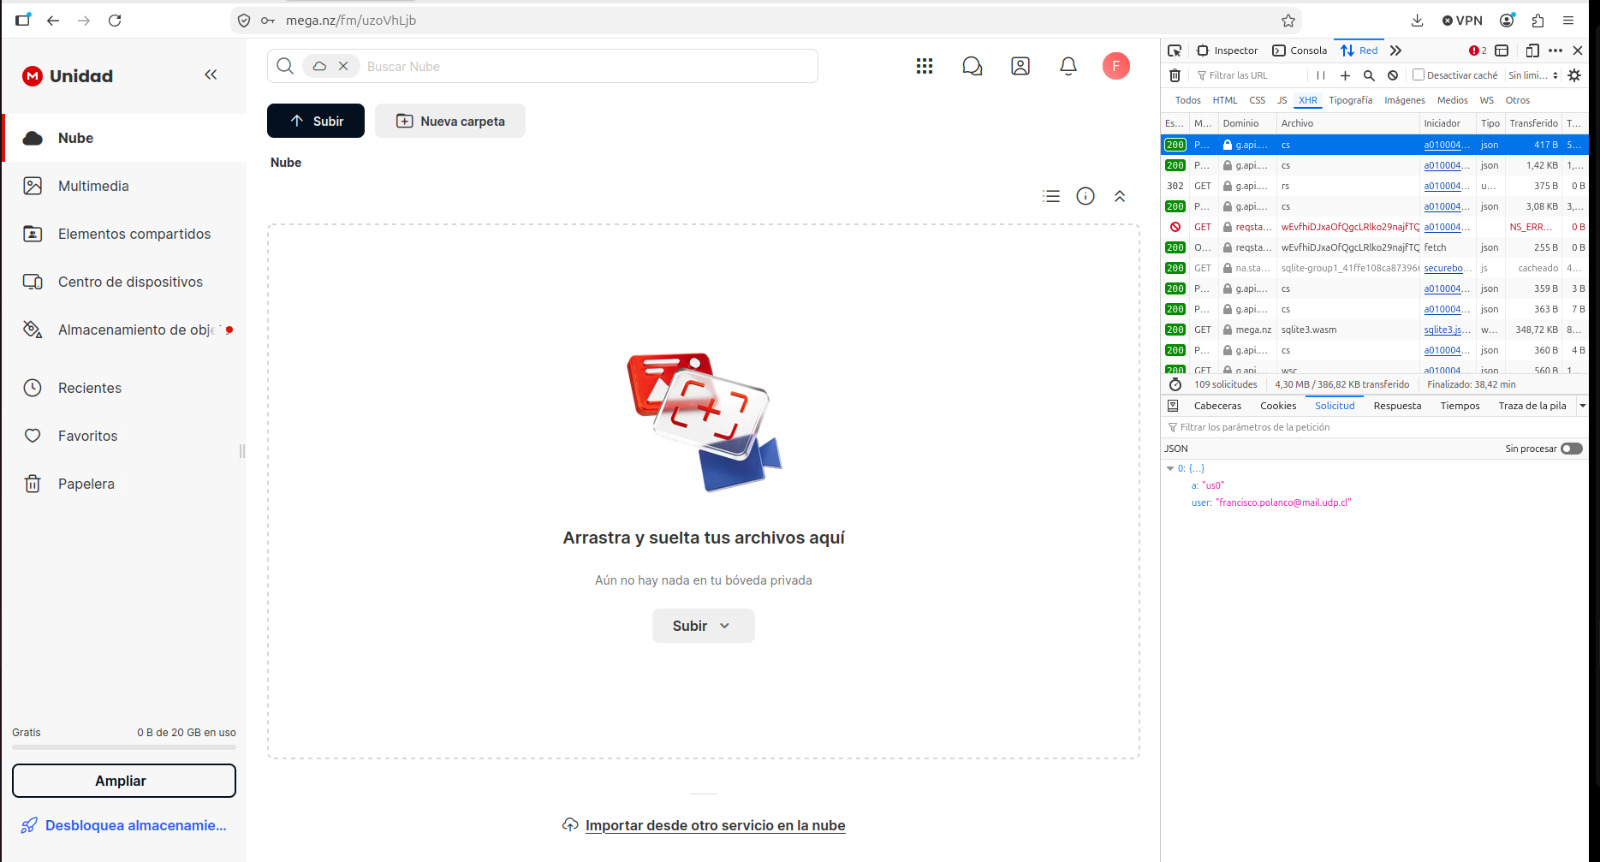
\includegraphics[width=0.85\textwidth]{fig05_login_us0_request_orig.jpeg}
            \caption{Captura original.}
        \end{subfigure}
        \vspace{0.4cm}
        \begin{subfigure}[b]{\textwidth}
            \centering
            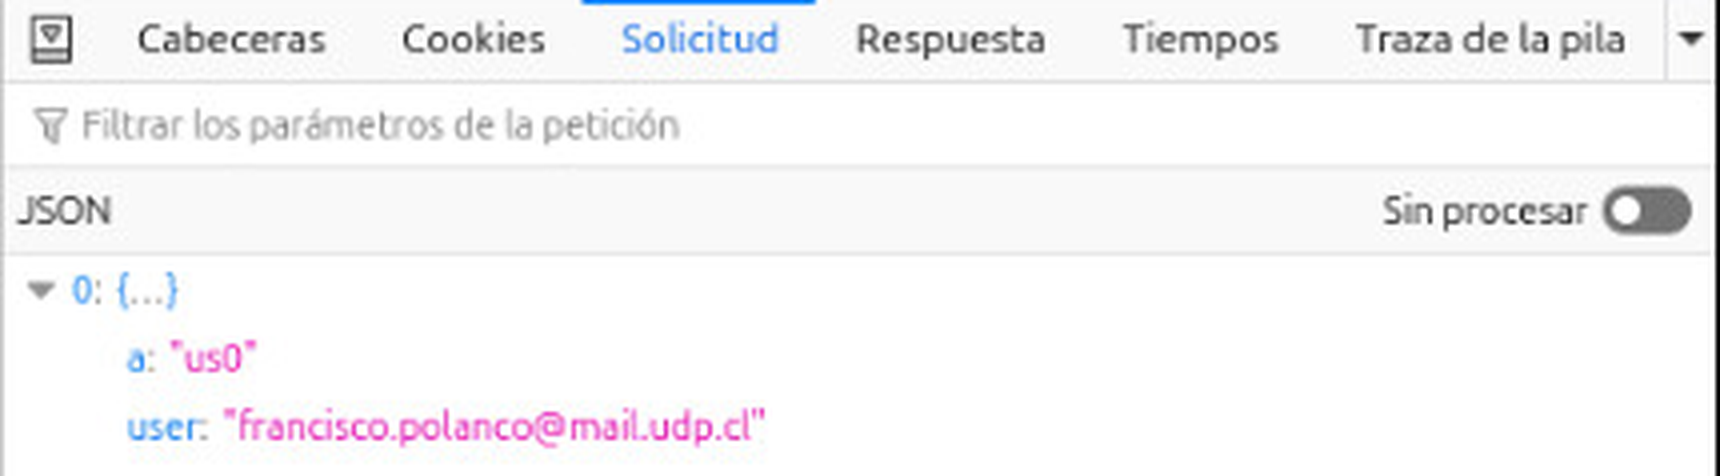
\includegraphics[width=0.85\textwidth]{fig05_login_us0_request_recorte.png}
            \caption{Recorte ampliado para mayor legibilidad.}
        \end{subfigure}
        \caption{Solicitud \texttt{a: "us0"} enviada al iniciar sesión, en la que el cliente solicita el salt asociado a la cuenta.}
        \label{fig:login-us0-req}
    \end{figure}

    El cuerpo JSON de esta solicitud es el siguiente:
\begin{lstlisting}[language=json]
{
  "a": "us0",
  "user": "francisco.polanco@mail.udp.cl"
}
\end{lstlisting}

    El campo \texttt{a} tiene el valor \texttt{"us0"} (\textit{user session, paso 0}), la acción que inicia el flujo de login pidiendo los parámetros necesarios para derivar la contraseña, antes de cualquier intento de autenticación real; y el campo \texttt{user} es el correo electrónico con el que se identifica la cuenta, el único dato que el cliente necesita entregar en este primer paso para que el servidor sepa a qué cuenta corresponde el salt solicitado. Nótese que en ningún momento de esta solicitud se envía la contraseña ni ningún valor derivado de ella, ya que el navegador todavía no cuenta con el salt necesario para calcularlo.

    \item \textbf{Respuesta del servidor:} con el correo ya identificado, el servidor responde entregando el salt solicitado en el paquete anterior, con esto ya se puede construir la contraseña para acceder a la cuenta. La Figura~\ref{fig:login-us0-resp} muestra esta respuesta.

    \begin{figure}[H]
        \centering
        \begin{subfigure}[b]{\textwidth}
            \centering
            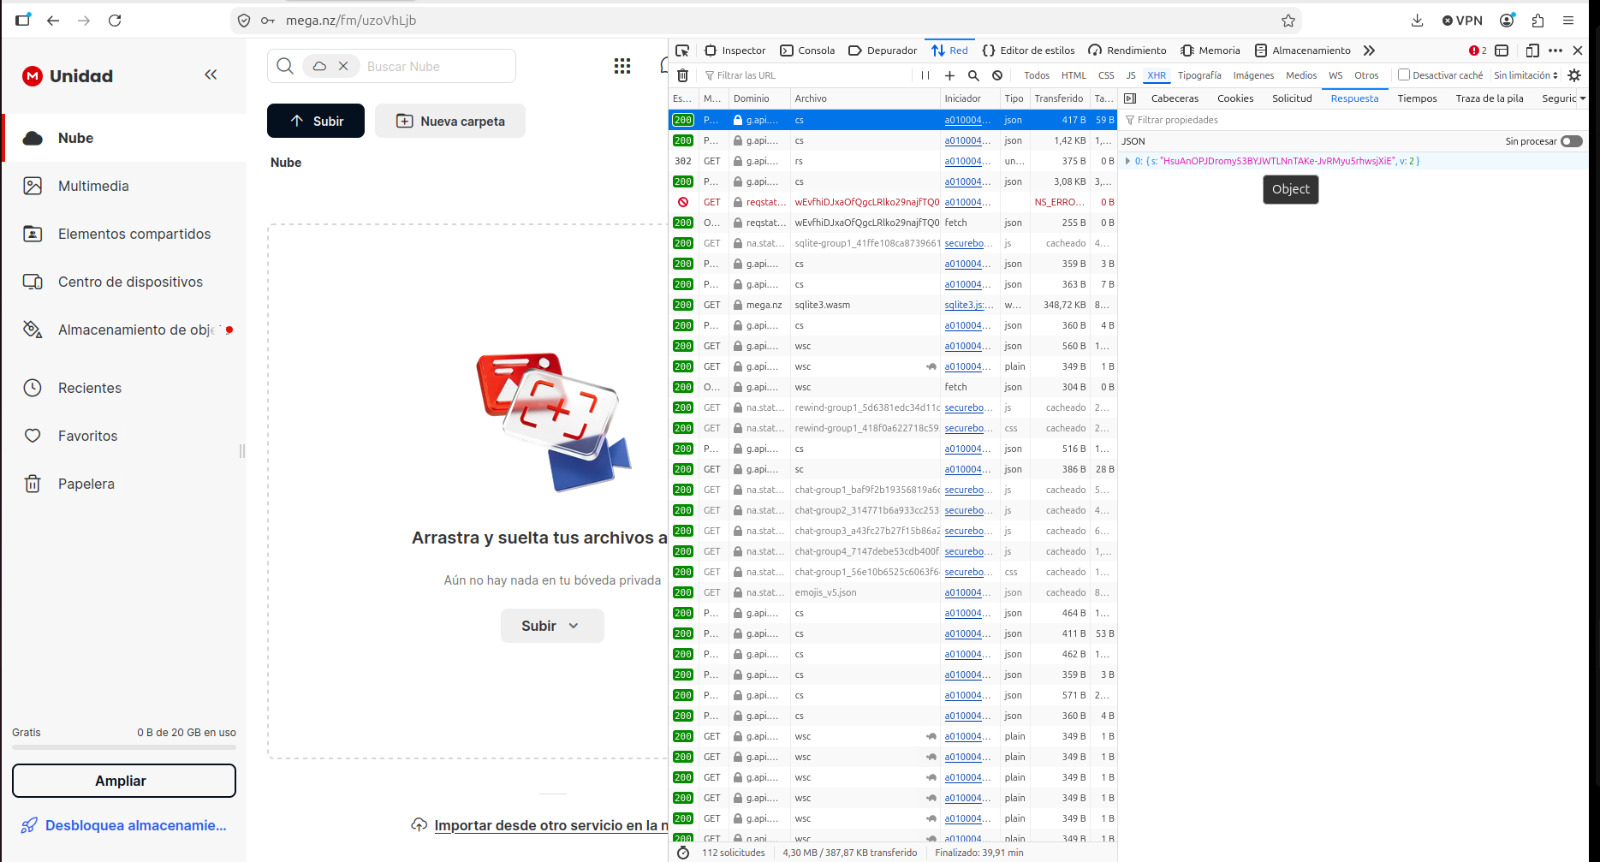
\includegraphics[width=0.85\textwidth]{fig06_login_us0_response_orig.jpeg}
            \caption{Captura original.}
        \end{subfigure}
        \vspace{0.4cm}
        \begin{subfigure}[b]{\textwidth}
            \centering
            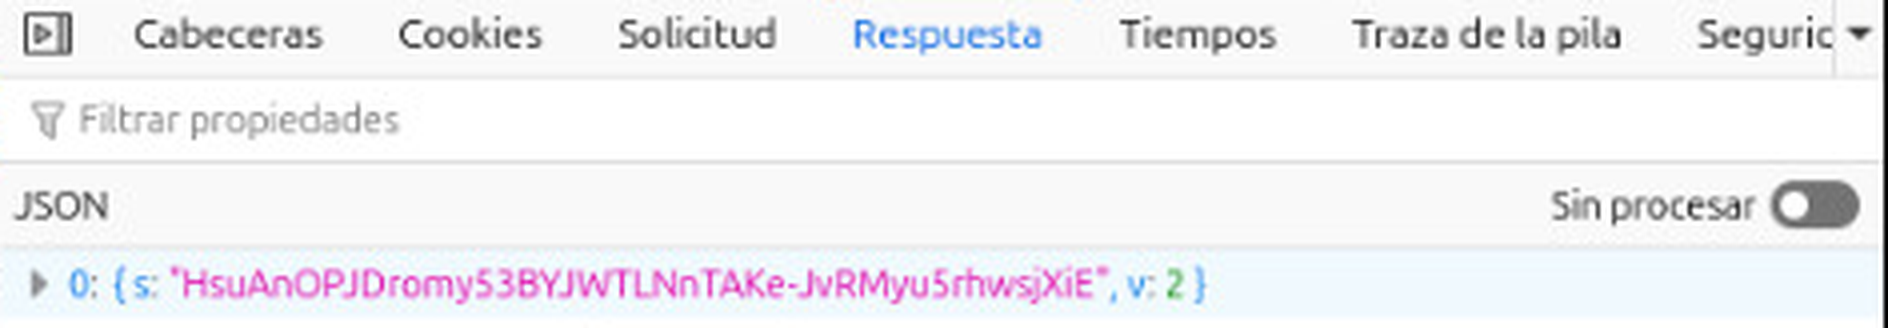
\includegraphics[width=0.85\textwidth]{fig06_login_us0_response_recorte.png}
            \caption{Recorte ampliado para mayor legibilidad.}
        \end{subfigure}
        \caption{Respuesta del servidor a \texttt{us0}, con el salt (\texttt{s}) de la cuenta y el indicador de versión (\texttt{v: 2}).}
        \label{fig:login-us0-resp}
    \end{figure}

    El cuerpo JSON de la respuesta es el siguiente:
\begin{lstlisting}[language=json]
{
  "s": "HsuAnOPJDromy53BYJWTLNnTAKe-JvRMyu5rhwsjXiE",
  "v": 2
}
\end{lstlisting}

    El campo \texttt{s} es el \textbf{salt} de la cuenta: un valor aleatorio, único para cada usuario, que el servidor generó y almacenó en el momento del registro, y que ahora reutiliza en cada inicio de sesión. Su función es evitar que dos usuarios con la misma contraseña obtengan el mismo resultado al derivarla, y, sobre todo, impedir que un atacante precalcule tablas de hashes (\textit{rainbow tables}) válidas para muchas cuentas. El campo \texttt{v}, con valor \textbf{2}, confirma que esta cuenta sigue reconocida bajo el esquema de cuentas versión 2 visto durante el registro (Sección~\ref{sec:registro}), es decir, que la derivación de la contraseña debe hacerse mediante PBKDF2 con HMAC-SHA512: un algoritmo que, en lugar de aplicar la función de hash una sola vez, la repite miles de veces para encarecer deliberadamente el cálculo y hacer mucho más lento un ataque de fuerza bruta.

    \item \textbf{Solicitud 2 — envío del hash de autenticación (\texttt{a: "us"})}: con el salt ya calculado, el navegador recién en este punto puede calcular el valor que realmente demuestra el conocimiento de la contraseña. La Figura~\ref{fig:login-us-req} muestra la solicitud enviada inmediatamente después de ese cálculo, es decir, el momento en que el cliente intenta autenticarse ante el servidor.

    \begin{figure}[H]
        \centering
        \begin{subfigure}[b]{\textwidth}
            \centering
            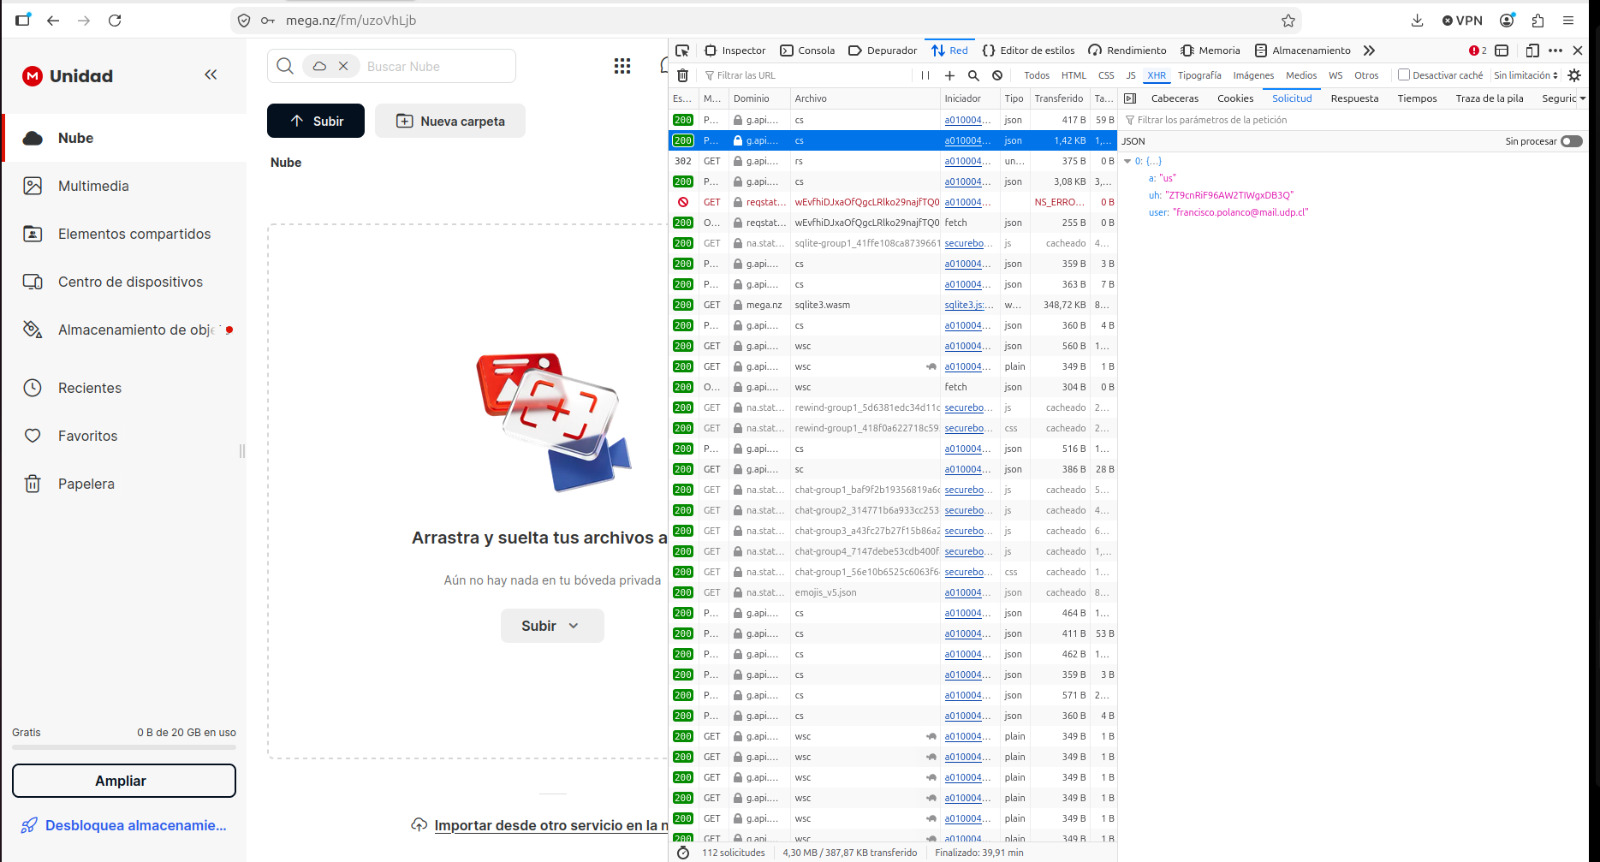
\includegraphics[width=0.85\textwidth]{fig07_login_us_request_orig.jpeg}
            \caption{Captura original.}
        \end{subfigure}
        \vspace{0.4cm}
        \begin{subfigure}[b]{\textwidth}
            \centering
            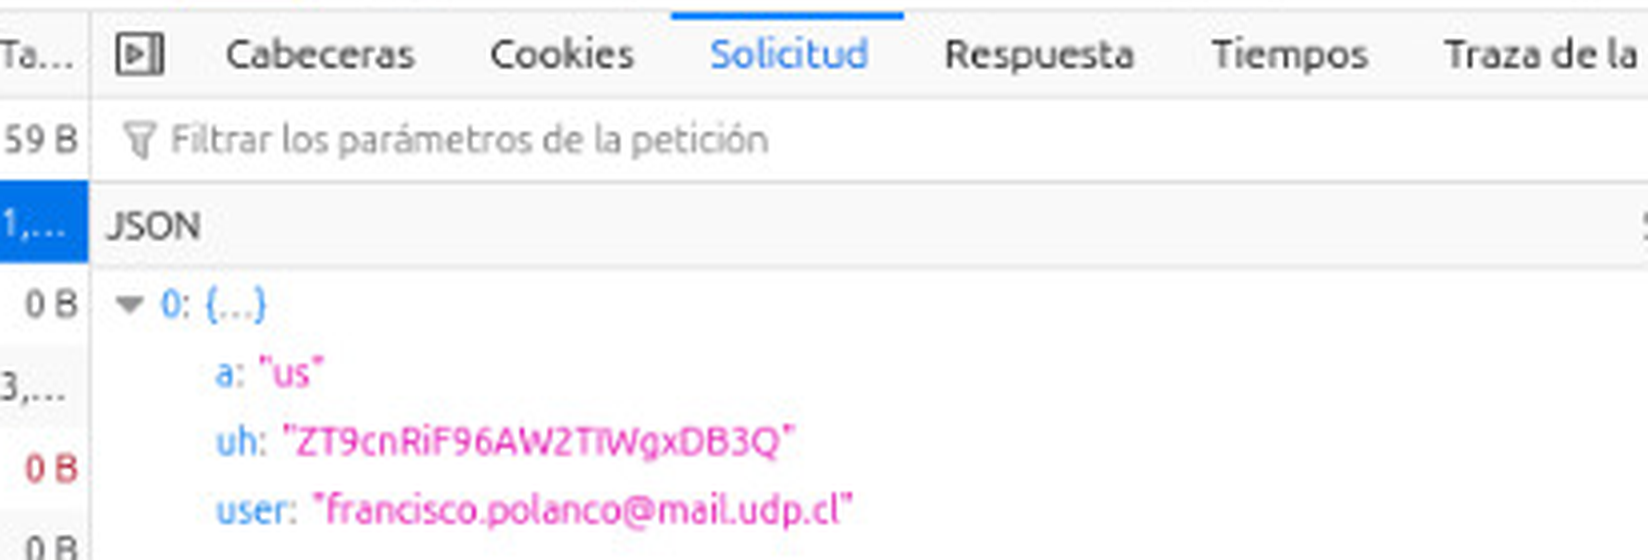
\includegraphics[width=0.85\textwidth]{fig07_login_us_request_recorte.png}
            \caption{Recorte ampliado para mayor legibilidad.}
        \end{subfigure}
        \caption{Solicitud \texttt{a: "us"} con el \textit{user hash} (\texttt{uh}) calculado por el cliente a partir de la contraseña y el salt.}
        \label{fig:login-us-req}
    \end{figure}

    El cuerpo JSON de esta solicitud es el siguiente:
\begin{lstlisting}[language=json]
{
  "a": "us",
  "uh": "ZT9cnRiF96AW2TIWgxDB3Q",
  "user": "francisco.polanco@mail.udp.cl"
}
\end{lstlisting}

    El campo \texttt{"a"} cambia a \texttt{"us"} (\textit{user session}), la acción que indica al servidor que esta vez sí se trata de un intento real de autenticación, a diferencia de \texttt{"us0"} que solo pedía datos previos; \texttt{user} vuelve a identificar la cuenta mediante el correo electrónico; y \texttt{uh} (\textit{user hash}) es el campo central de esta solicitud: el resultado de aplicar PBKDF2-HMAC-SHA512 a la contraseña ingresada por el usuario, usando como salt el valor \texttt{s} recibido en el paso anterior (el detalle exacto de iteraciones y longitud de clave se reproduce y verifica en la Sección~\ref{sec:consola}). Este cálculo se realiza completamente en el navegador, de modo que la contraseña en texto plano nunca sale del equipo del usuario: lo único que viaja por la red es \texttt{uh}, que es precisamente el valor que el servidor compara contra el que guardó al momento del registro para decidir si la autenticación es válida.

    Para completar la secuencia, la Figura~\ref{fig:login-us-resp} muestra la respuesta que entrega el servidor una vez que valida ese \texttt{uh} como correcto:

    \begin{figure}[H]
        \centering
        \begin{subfigure}[b]{\textwidth}
            \centering
            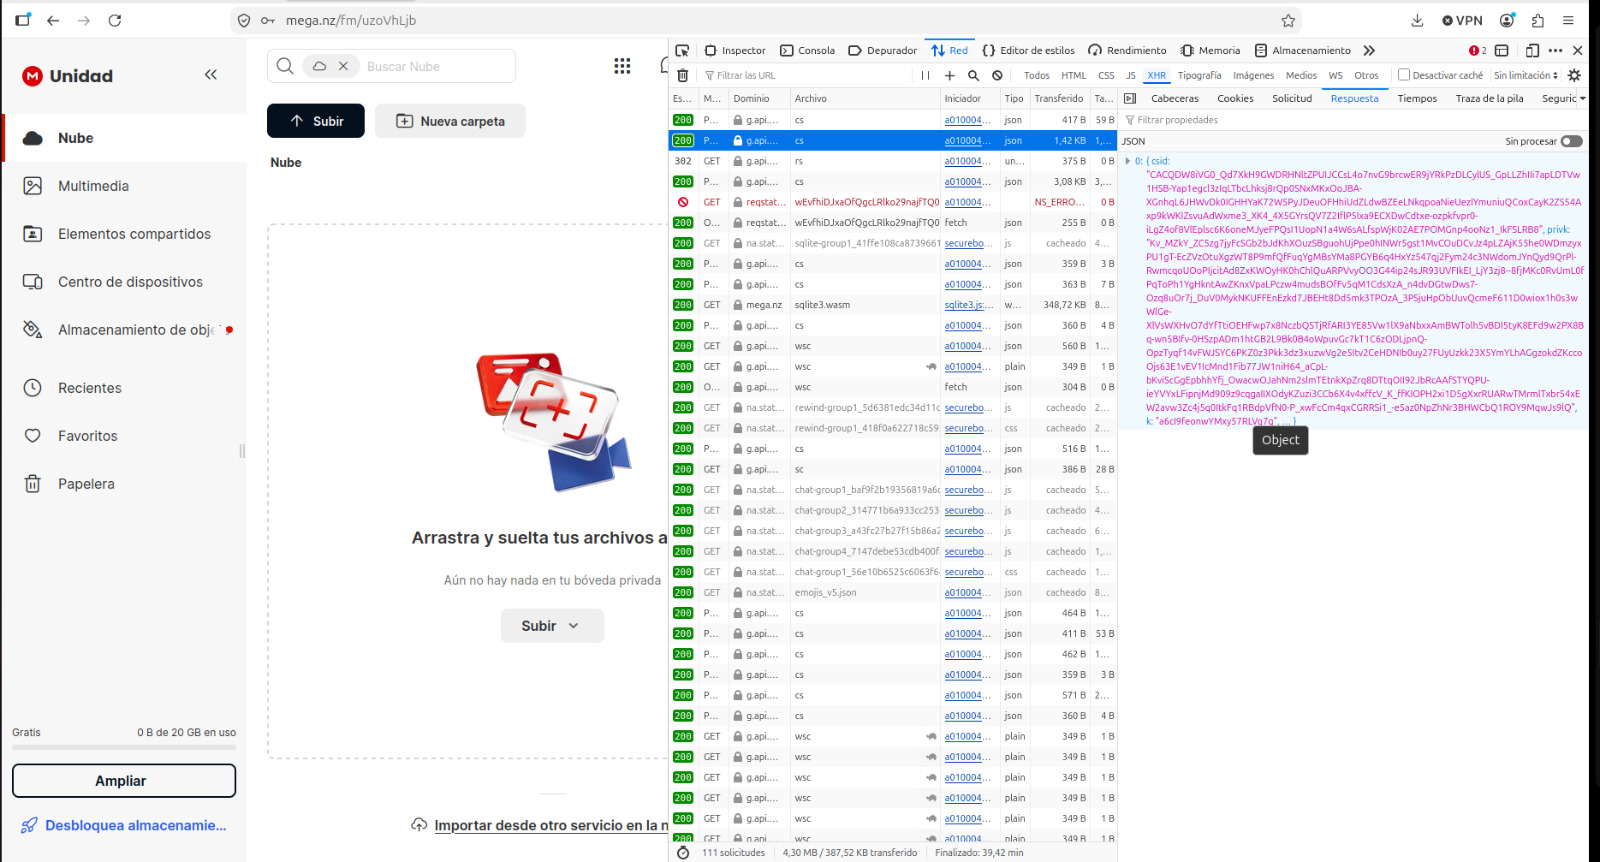
\includegraphics[width=0.85\textwidth]{fig08_login_us_response_csid_orig.jpeg}
            \caption{Captura original.}
        \end{subfigure}
        \vspace{0.4cm}
        \begin{subfigure}[b]{\textwidth}
            \centering
            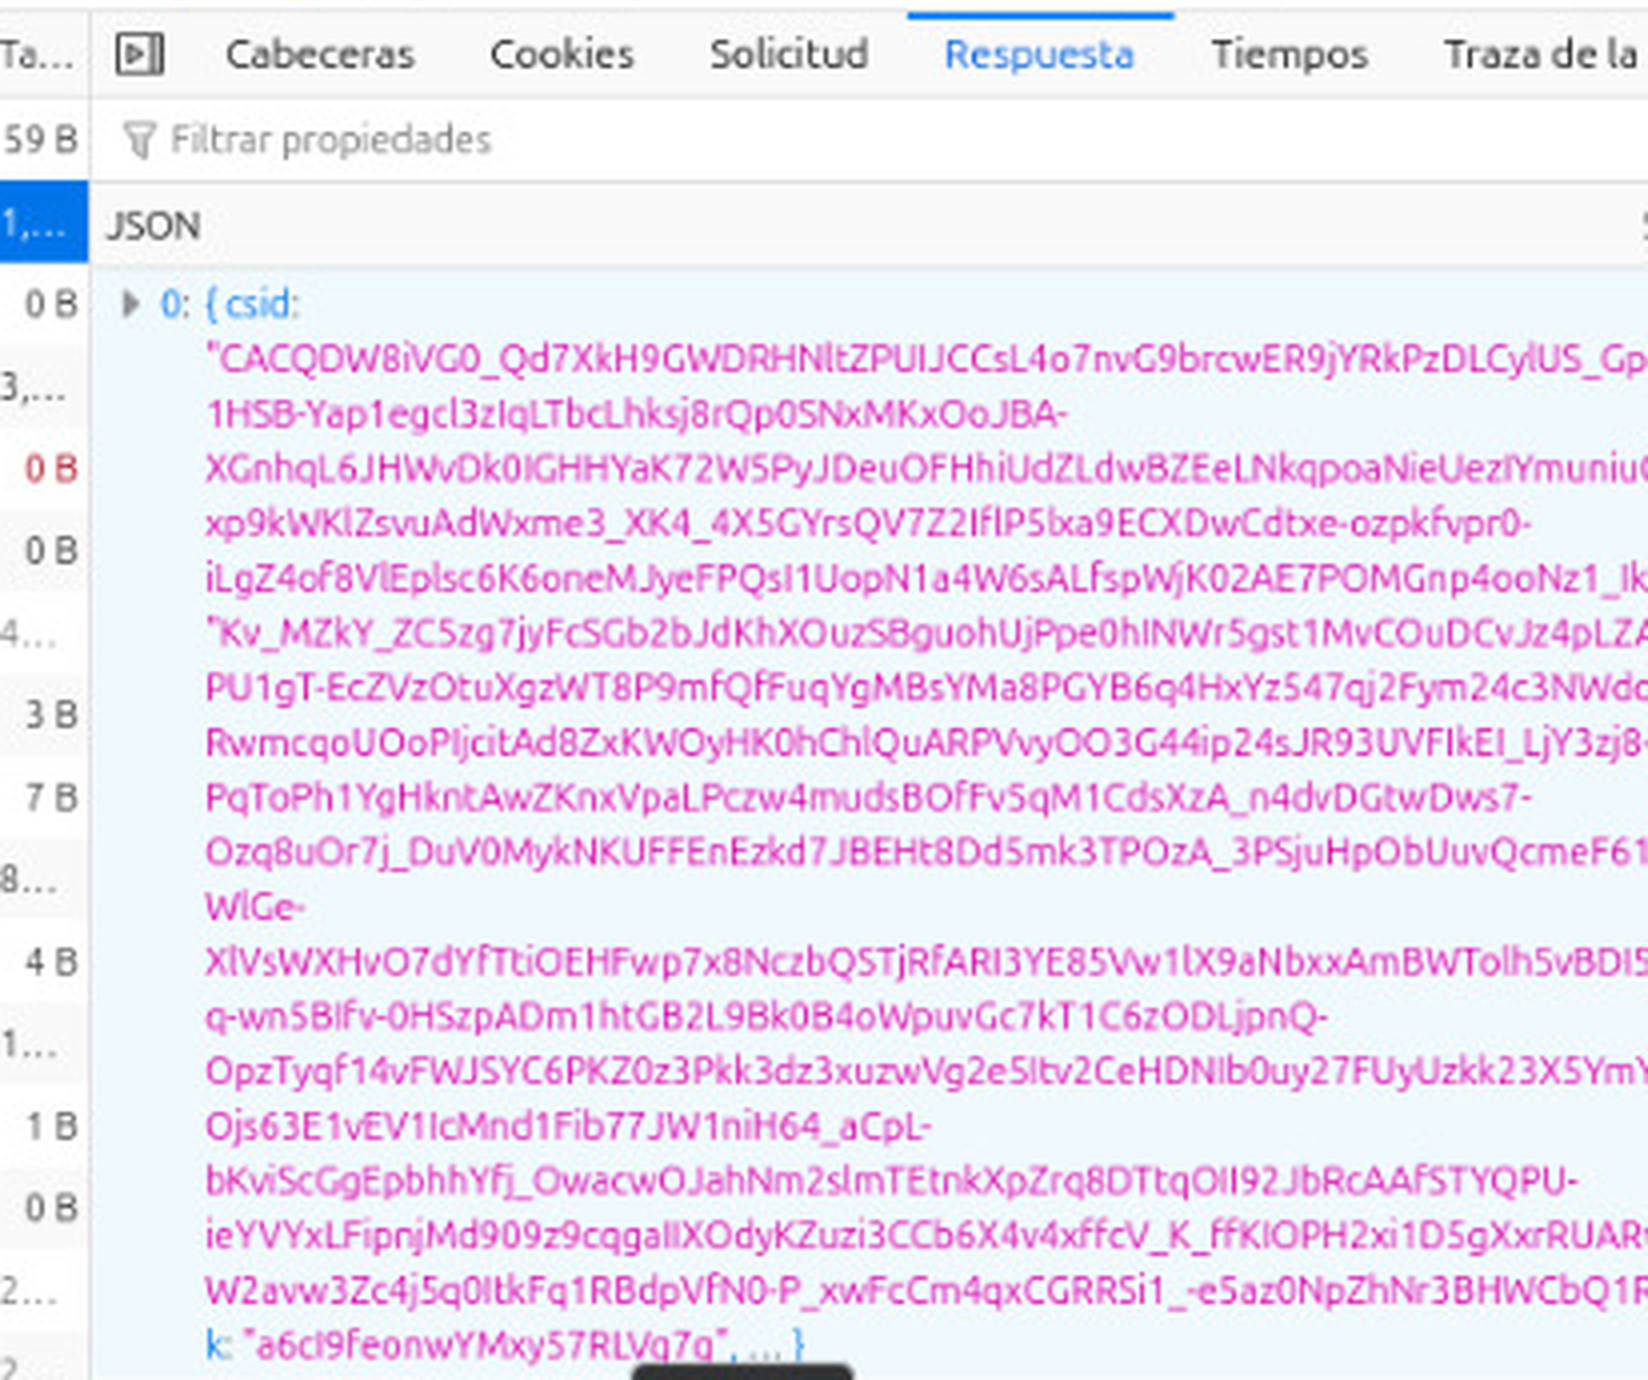
\includegraphics[width=0.85\textwidth]{fig08_login_us_response_csid_recorte.png}
            \caption{Recorte ampliado para mayor legibilidad.}
        \end{subfigure}
        \caption{Respuesta del servidor ante un \texttt{uh} válido: sesión autenticada (\texttt{csid}) y material cifrado de la cuenta.}
        \label{fig:login-us-resp}
    \end{figure}

    Esta respuesta incluye un \texttt{csid} (\textit{session ID}), el identificador de sesión que el servidor entrega solo cuando el \texttt{uh} recibido coincide con el que tiene almacenado, junto con el material cifrado de la cuenta (\textit{master key} y clave privada) que el navegador necesitará descifrar a continuación usando la \textit{password key} derivada de la contraseña real. Toda la secuencia de login confirma así, de extremo a extremo, que la autenticación depende exclusivamente de un valor derivado mediante PBKDF2-HMAC-SHA512 (\texttt{uh}), y que la contraseña en texto plano no se transmite en ningún punto del proceso.
\end{itemize}

\subsection{Genera el hash de la contraseña desde la consola del navegador}
\label{sec:consola}

\sangria Para reproducir el valor de autenticación se comenzó por inspeccionar las funciones criptográficas disponibles en el código JavaScript de la página. Esta búsqueda era necesaria porque encontrar una función que procese contraseñas no basta para demostrar que sea la utilizada por la cuenta, ya que Mega mantiene compatibilidad con más de una versión de su esquema de autenticación. Durante la inspección se identificaron las siguientes funciones asociadas al mecanismo antiguo (v1):


\begin{figure}[H]
    \centering
    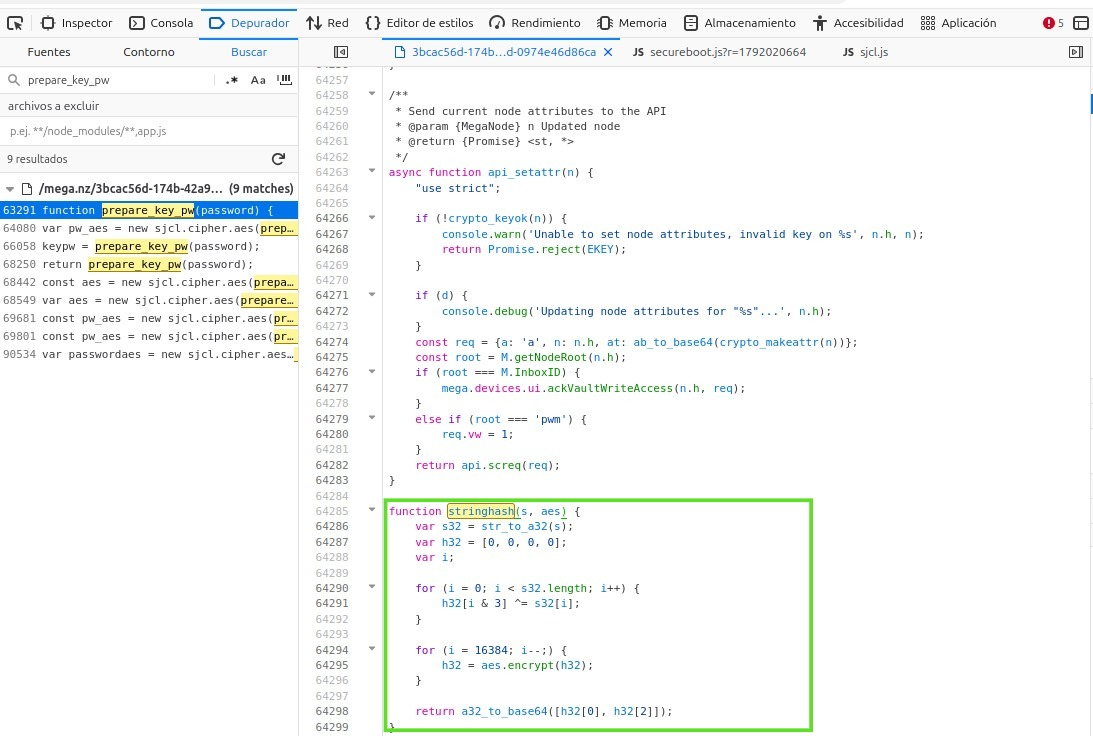
\includegraphics[width=1\linewidth]{figuras/Generador_contraseña.jpeg}
    \caption{Función con algoritmo de cifrado}
    \label{fig:fn-generador}
\end{figure}
\begin{figure}[H]
    \centering
    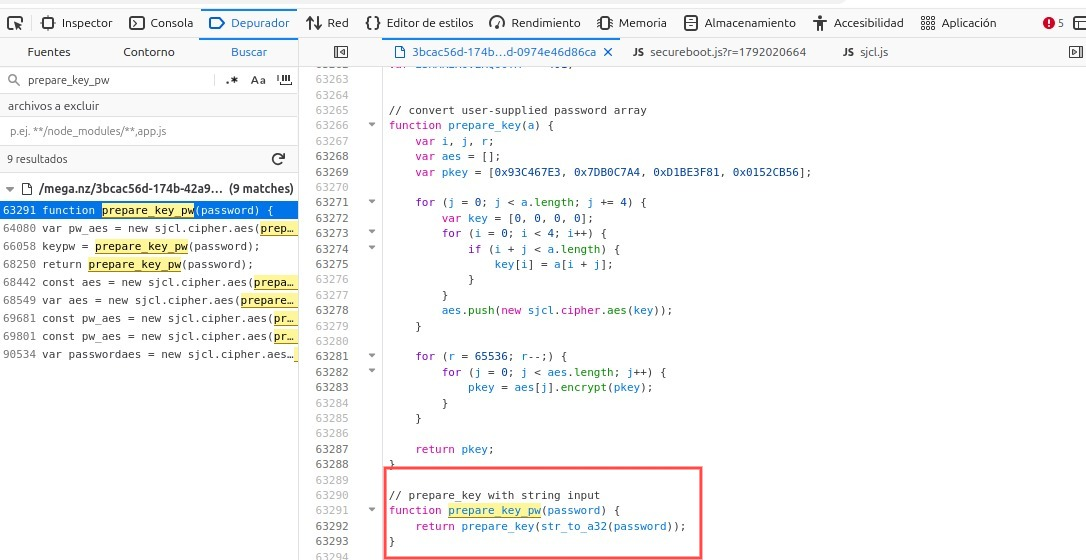
\includegraphics[width=1\linewidth]{figuras/Invocador_contraseña.jpeg}
    \caption{Función para crear contraseña}
    \label{fig:fn-invocador}
\end{figure}
Estas funciones aplican 16.384/65.536 rondas de cifrado AES-ECB sobre la contraseña, correspondientes al algoritmo propietario usado por cuentas antiguas (v1). Sin embargo, dado que las cuentas actuales utilizan: \textbf{v2}, estas funciones no corresponden al algoritmo realmente utilizado para autenticar la cuenta, aunque permanecen cargadas en el cliente por compatibilidad con cuentas antiguas.

Inspeccionando el código fuente cargado por el navegador, se confirmó la presencia de la librería SJCL (Stanford JavaScript Crypto Library), que implementa \texttt{sjcl.misc.pbkdf2}. Con esto se confirmaron los parámetros exactos utilizados por las cuentas v2:

\begin{itemize}
    \item Algoritmo: \textbf{PBKDF2}
    \item Función pseudoaleatoria: \textbf{HMAC-SHA512}
    \item Iteraciones: \textbf{100.000}
    \item Longitud de clave derivada: 256 bits (32 bytes), divididos en dos mitades de 16 bytes cada una: los primeros 16 bytes forman la \textit{password key} (usada para cifrar/descifrar la \textit{master key}), y los últimos 16 bytes forman el \textbf{user hash (\texttt{uh})} enviado al servidor para autenticarse.
\end{itemize}

Para comprobar esto de forma práctica, se replicó el cálculo directamente desde la consola del navegador utilizando la Web Crypto API nativa, partiendo de la contraseña en texto plano y el salt (\texttt{s}) obtenido previamente en la respuesta de la solicitud \texttt{us0}. 




\begin{lstlisting}[language=java]
async function calcularUh(password, saltBase64url) {
  const salt = Uint8Array.from(
    atob(saltBase64url.replace(/-/g,'+').replace(/_/g,'/')),
    c => c.charCodeAt(0)
  );

  const keyMaterial = await crypto.subtle.importKey(
    "raw", new TextEncoder().encode(password), "PBKDF2", false, ["deriveBits"]
  );

  const derivedBits = await crypto.subtle.deriveBits(
    { name: "PBKDF2", salt: salt, iterations: 100000, hash: "SHA-512" },
    keyMaterial, 256
  );

  const bytes = new Uint8Array(derivedBits);
  const passwordKey = bytes.slice(0, 16);
  const userHashBytes = bytes.slice(16, 32);

  function toBase64url(arr) {
    let bin = '';
    arr.forEach(b => bin += String.fromCharCode(b));
    return btoa(bin).replace(/\+/g,'-').replace(/\//g,'_').replace(/=+$/,'');
  }

  return { passwordKey: toBase64url(passwordKey), userHash: toBase64url(userHashBytes) };
}

calcularUh("Laboratorio3. (Clave utilizada)", "HsuAnOPJDromy53BYJWTLNnTAKe-JvRMyu5rhwsjXiE")
  .then(r => console.log("RESULTADO:", r));
\end{lstlisting}

Esta función toma la contraseña en texto plano y el salt recibido del servidor, deriva 256 bits mediante PBKDF2-HMAC-SHA512 con 100.000 iteraciones, y divide el resultado en las dos mitades descritas anteriormente (\texttt{passwordKey} y \texttt{userHash}), codificándolas en Base64url para que puedan compararse directamente con los valores observados en el tráfico real.

Al ejecutar este código con la contraseña real de la cuenta, se obtuvo el resultado mostrado en detalle en la Figura~\ref{fig:consola-resultado}, donde se aprecia de cerca la salida impresa en la consola tras invocar la función:

\begin{figure}[H]
    \centering
    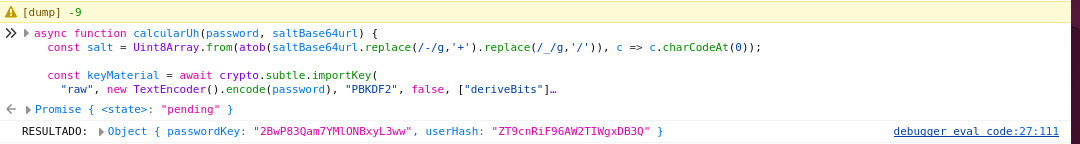
\includegraphics[width=0.95\textwidth]{fig10_consola_resultado_zoom.jpeg}
    \caption{Resultado de \texttt{calcularUh}}
    \label{fig:consola-resultado}
\end{figure}

El resultado obtenido, tal como aparece en la figura, es el siguiente:

\begin{lstlisting}[language=json]
RESULTADO: {
  passwordKey: "2BwP83Qam7YMlONBxyL3ww",
  userHash:    "ZT9cnRiF96AW2TIWgxDB3Q"
}
\end{lstlisting}

El valor \texttt{userHash} calculado manualmente desde la consola del navegador coincide exactamente con el valor \texttt{uh} capturado previamente en la solicitud real de login: \texttt{ZT9cnRiF96AW2TIWgxDB3Q}. Esta coincidencia exacta confirma, de manera práctica y reproducible, que el algoritmo identificado (PBKDF2-HMAC-SHA512 con 100.000 iteraciones) es efectivamente el utilizado por Mega para autenticar cuentas versión 2.

\subsection{Intercepta el tráfico login con BurpSuite}
\label{sec:burp}

\sangria La siguiente etapa consistió en observar el mismo inicio de sesión desde una herramienta distinta de las funciones de desarrollador. Para ello se configuró BurpSuite como proxy local en Firefox. El propósito fue detener las peticiones antes de su envío, inspeccionar su contenido y poder modificar las peticiones para la prueba posterior. La preparación del entorno se realizó de la siguiente manera:

\begin{enumerate}
    \item Se inició BurpSuite con un proyecto temporal y configuración por defecto, dejando el proxy escuchando en \texttt{127.0.0.1:8080}.
    \item Se configuró Firefox para utilizar dicho proxy manualmente (HTTP y HTTPS) en \textit{Configuración de red}.
    \item Se instaló el certificado CA de BurpSuite (descargado desde \texttt{http://burp}) en el almacén de autoridades de certificación de Firefox, habilitando la confianza para identificar sitios web. Esto permite interceptar tráfico HTTPS sin errores de certificado.
    \item Se verificó la correcta intercepción navegando a \texttt{https://mega.nz} con \textit{Intercept} desactivado, confirmando que el tráfico aparecía en Proxy \textrightarrow{} HTTP sin afectar la carga normal de la página.
\end{enumerate}

Posteriormente, se activó nuevamente Intercept is on y se repitió el proceso de inicio de sesión en \texttt{https://mega.nz/login}, utilizando la misma contraseña de la cuenta utilizada durante todo el laboratorio. La Figura~\ref{fig:burp-us} muestra la solicitud de autenticación real interceptada por BurpSuite, capturada desde el propio equipo hacia la API de Mega una vez que el navegador ya calculó el hash de la contraseña:

\clearpage
\begin{figure}[H]
    \centering
    \begin{subfigure}[b]{\textwidth}
        \centering
        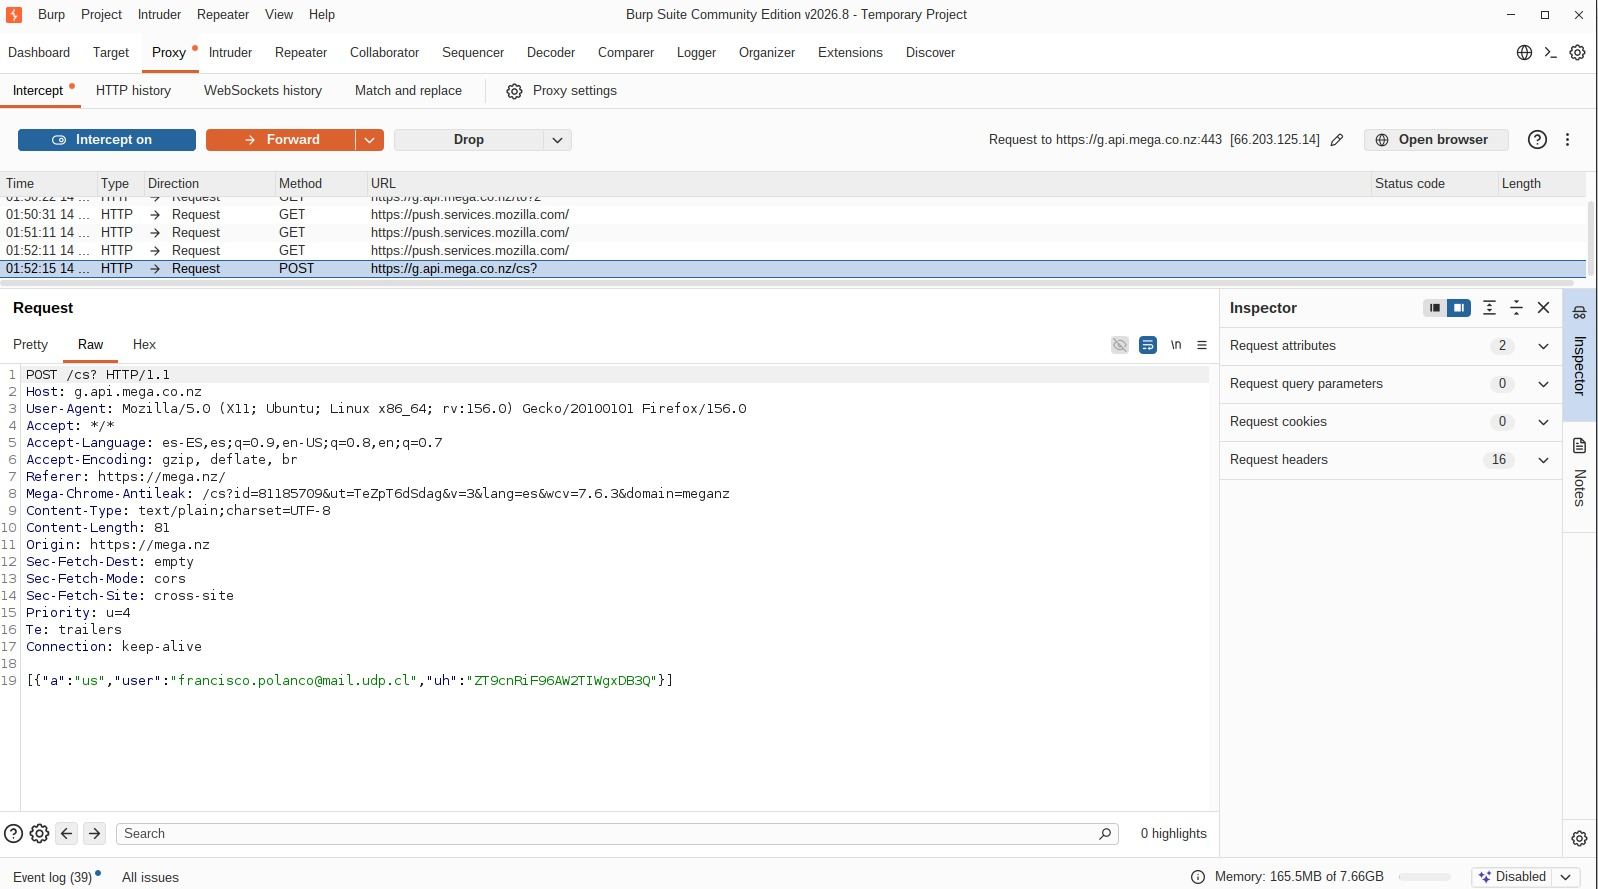
\includegraphics[width=0.85\textwidth,height=0.22\textheight,keepaspectratio]{fig12_burp_us_intercept_orig.jpeg}
        \caption{Captura original.}
    \end{subfigure}
    \vspace{0.3cm}
    \begin{subfigure}[b]{\textwidth}
        \centering
        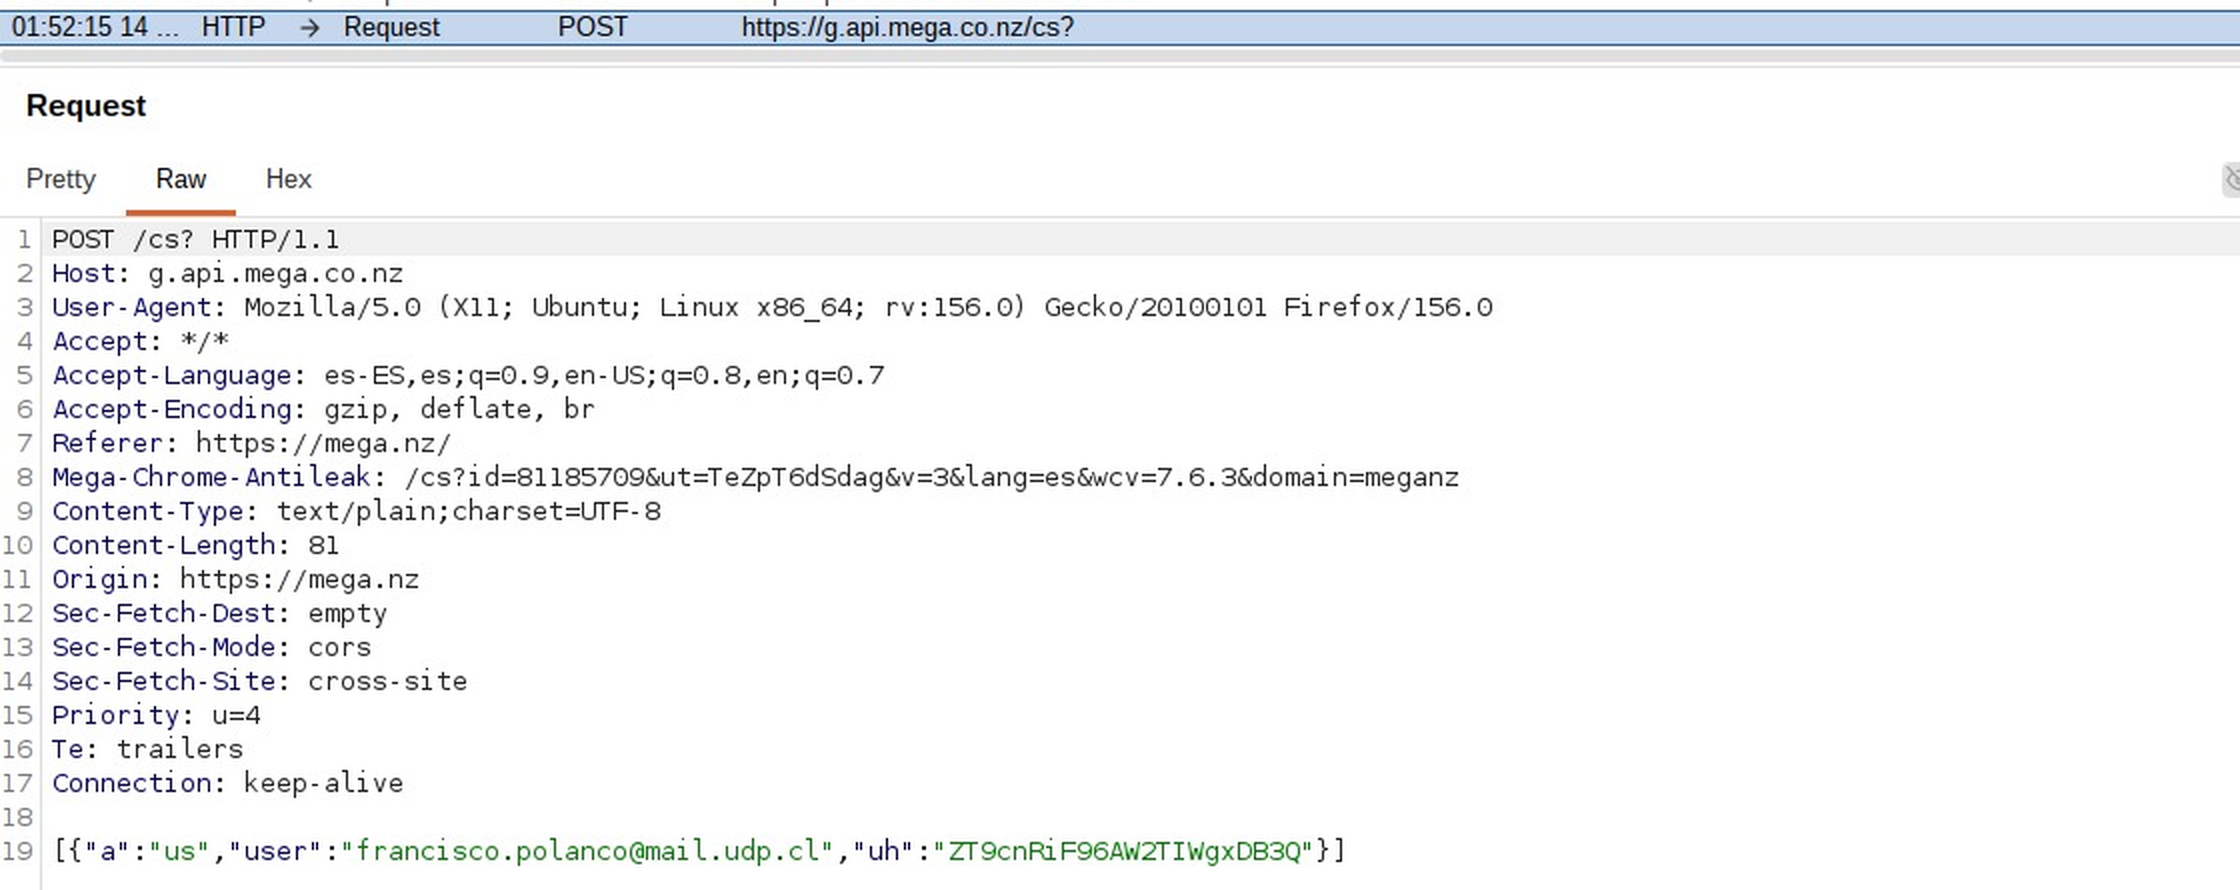
\includegraphics[width=0.85\textwidth,height=0.38\textheight,keepaspectratio]{fig12_burp_us_intercept_recorte.png}
        \caption{Recorte ampliado para mayor legibilidad.}
    \end{subfigure}
    \caption{Solicitud \texttt{"a": "us"} interceptada en BurpSuite}
    \label{fig:burp-us}
\end{figure}

La solicitud HTTP completa capturada en BurpSuite, correspondiente a lo mostrado en la figura anterior, fue la siguiente:

\begin{lstlisting}
POST /cs? HTTP/1.1
Host: g.api.mega.co.nz
User-Agent: Mozilla/5.0 (X11; Ubuntu; Linux x86_64; rv:156.0) Gecko/20100101 Firefox/156.0
Accept: */*
Accept-Language: es-ES,es;q=0.9,en-US;q=0.8,en;q=0.7
Accept-Encoding: gzip, deflate, br
Referer: https://mega.nz/
Content-Type: text/plain;charset=UTF-8
Origin: https://mega.nz
Connection: keep-alive

[{"a":"us","user":"francisco.polanco@mail.udp.cl","uh":"ZT9cnRiF96AW2TIWgxDB3Q"}]
\end{lstlisting}

Se observa que, al igual que en las capturas realizadas anteriormente, el campo \texttt{uh} enviado en el cuerpo de la solicitud corresponde al \textit{user hash} derivado mediante PBKDF2-HMAC-SHA512, y no a la contraseña en texto plano ni a un hash simple de ella. Esto permite comprobar, para las solicitudes capturadas durante la prueba, que no se envió la contraseña en texto plano: el cliente realiza todo el proceso criptográfico localmente antes de enviar la solicitud.

\subsection{Realiza el intento de login}
\label{sec:pth}

\sangria Con el valor \texttt{uh} válido ya identificado, se evaluó si el servidor aceptaba ese dato de autenticación aun cuando el navegador hubiese calculado originalmente otro valor a partir de una contraseña incorrecta. 

\textbf{Procedimiento realizado:}
\begin{enumerate}
    \item Se cerró la sesión activa en Mega.
    \item Con BurpSuite en modo \textit{Intercept on}, se inició el proceso de login ingresando una contraseña incorrecta en el formulario. La Figura~\ref{fig:pth-incorrecto} muestra el momento en que BurpSuite intercepta la solicitud generada por el navegador a partir de dicha contraseña incorrecta, antes de que sea reenviada al servidor.

    \begin{figure}[H]
        \centering
        \begin{subfigure}[b]{\textwidth}
            \centering
            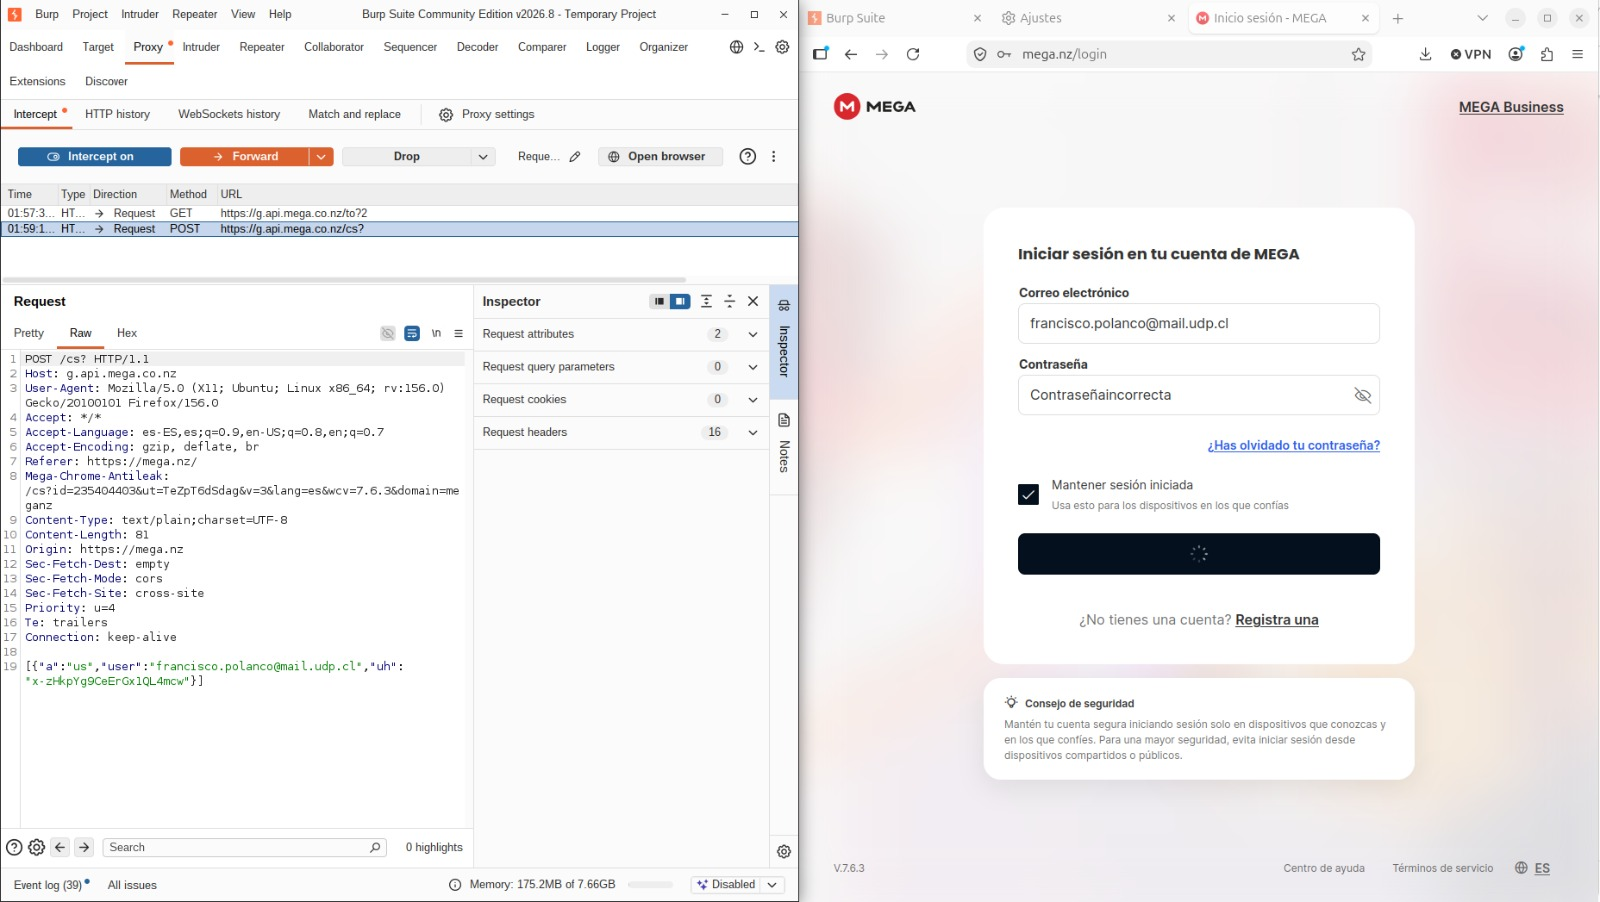
\includegraphics[width=0.7\textwidth]{fig13_pth_intento_incorrecto_orig.jpeg}
            \caption{Captura original.}
        \end{subfigure}
        \vspace{0.4cm}
        \begin{subfigure}[b]{\textwidth}
            \centering
            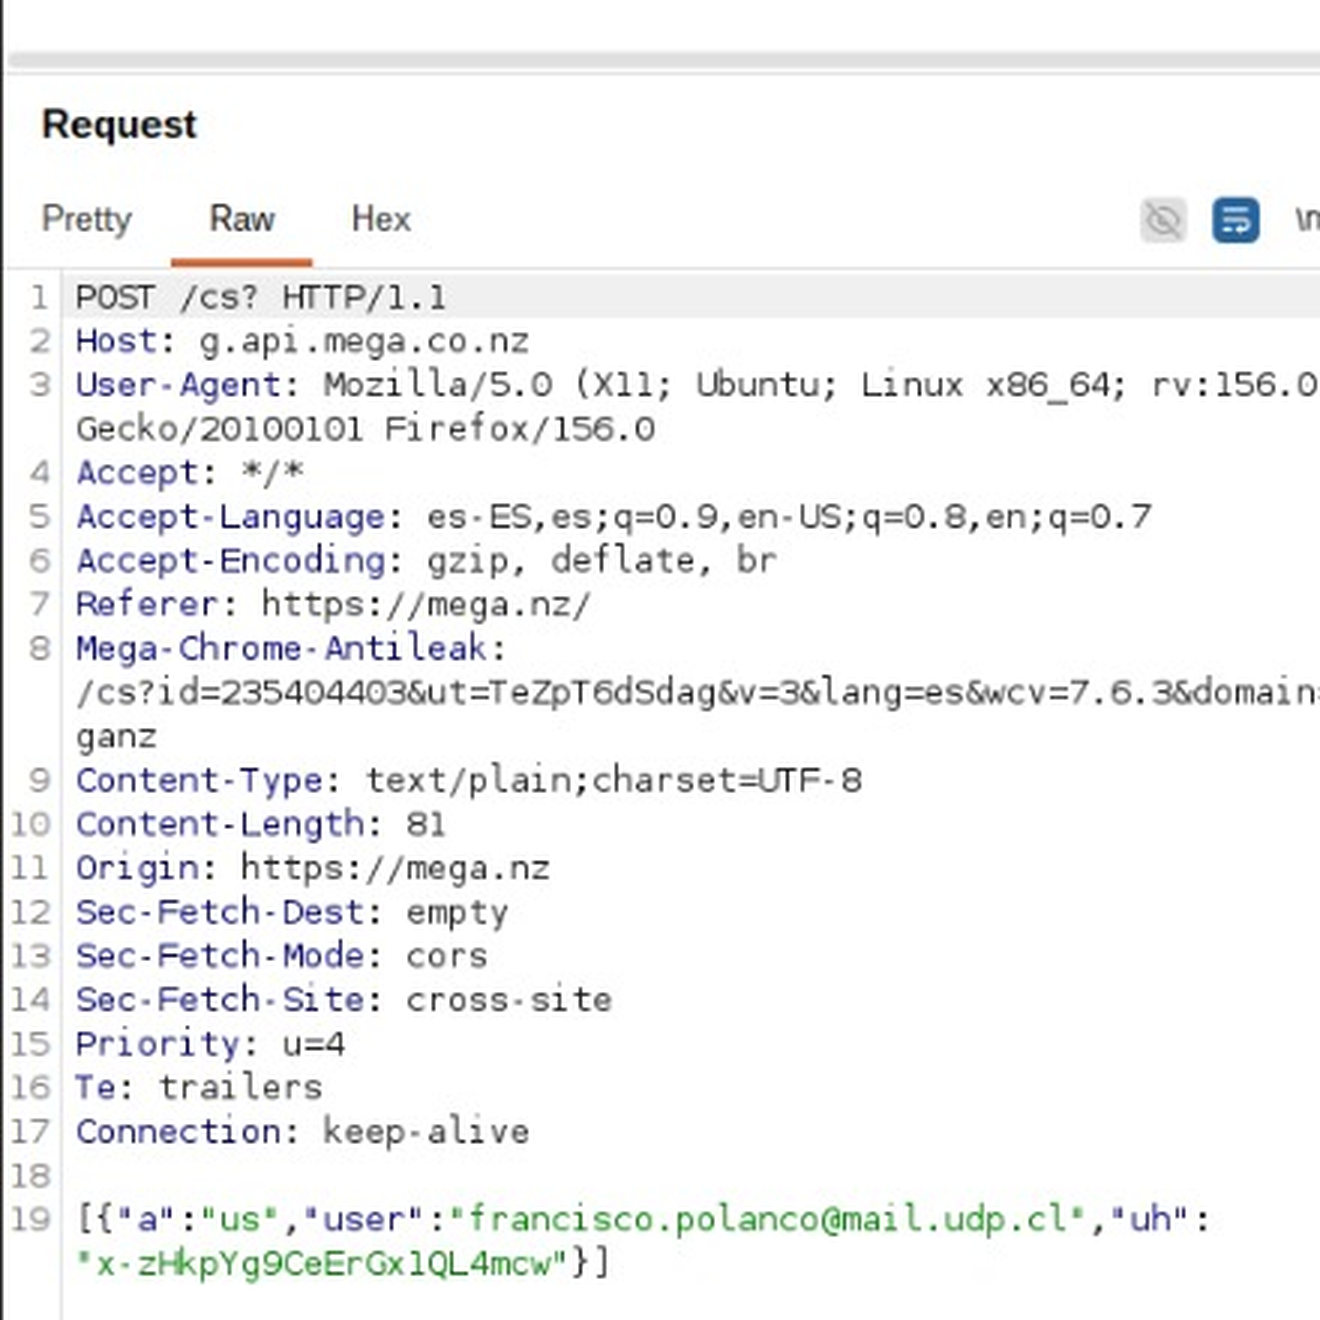
\includegraphics[width=0.7\textwidth]{fig13_pth_intento_incorrecto_recorte.png}
            \caption{Recorte ampliado para mayor legibilidad.}
        \end{subfigure}
        \caption{Intento de login con contraseña incorrecta: BurpSuite intercepta un \texttt{uh} inválido antes de su envío al servidor.}
        \label{fig:pth-incorrecto}
    \end{figure}

    El campo \texttt{uh} interceptado en esta solicitud (\texttt{x-zHkpYg9CeErGx1QL4mcw}) corresponde al hash calculado por el navegador a partir de la contraseña incorrecta, y por lo tanto \textbf{no coincide} con el valor válido obtenido en la Sección~\ref{sec:consola}.

    \item Se dejó pasar la primera solicitud (\texttt{a: "us0"}, solicitud del salt).
    \item Al interceptar la segunda solicitud (\texttt{a: "us"}), que contenía el \texttt{uh} inválido, se reemplazó manualmente dicho valor por el hash válido obtenido previamente (\texttt{ZT9cnRiF96AW2TIWgxDB3Q}). La Figura~\ref{fig:pth-modificacion} muestra el editor de BurpSuite en el momento exacto de ese reemplazo manual, antes de reenviar la solicitud.

    \begin{figure}[H]
        \centering
        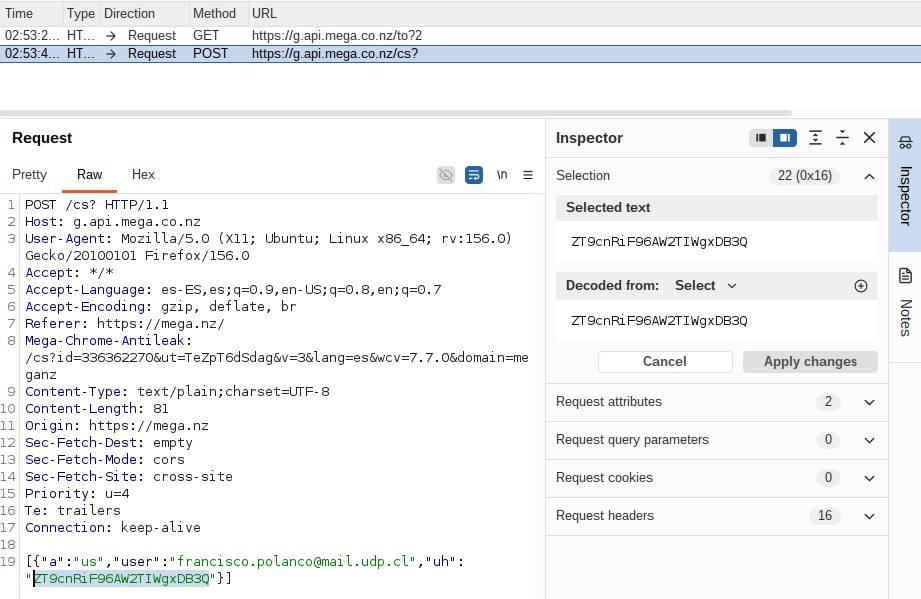
\includegraphics[width=0.95\textwidth]{fig14_pth_modificacion_uh.jpeg}
        \caption{Reemplazo manual del campo \texttt{uh} por el hash válido dentro de BurpSuite, antes de reenviar la solicitud.}
        \label{fig:pth-modificacion}
    \end{figure}

    \item Se reenvió (\textit{Forward}) la solicitud modificada.
\end{enumerate}

\textbf{Respuesta observada:} la Figura~\ref{fig:pth-respuesta} muestra la respuesta entregada por el servidor inmediatamente después de reenviar la petición con el \texttt{uh} modificado:

\begin{figure}[H]
    \centering
    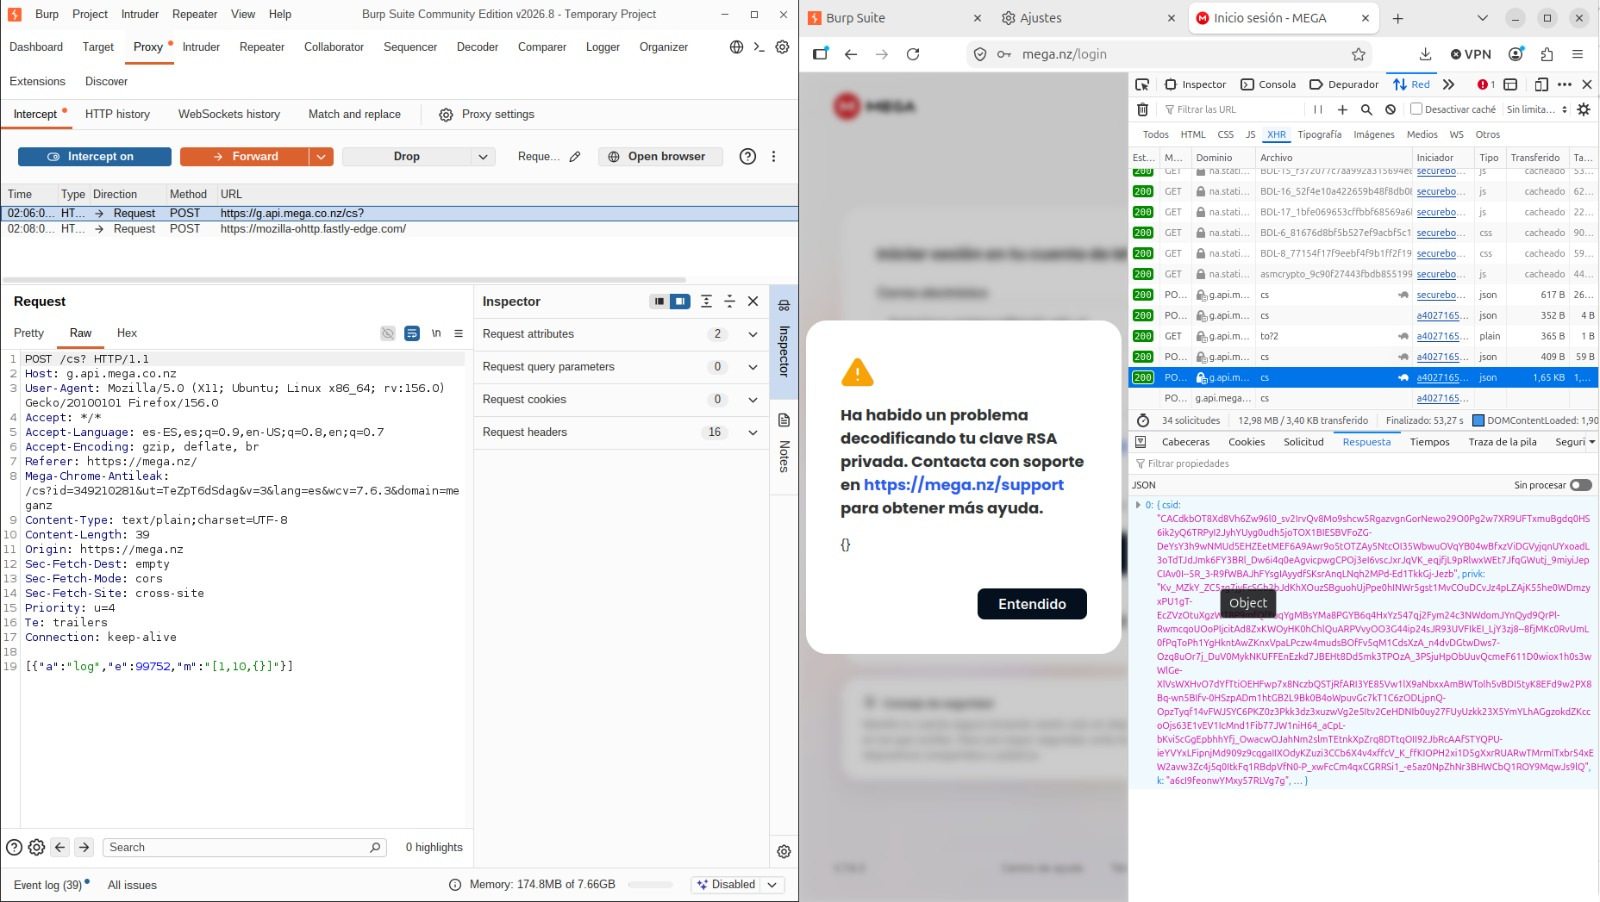
\includegraphics[width=0.95\textwidth]{fig16_pth_respuesta_csid.jpeg}
    \caption{Respuesta del servidor tras el ataque Pass the Hash: sesión autenticada (\texttt{csid}) obtenida sin conocer la contraseña real.}
    \label{fig:pth-respuesta}
\end{figure}

El cuerpo de la respuesta, visible en la figura anterior, incluía el identificador de sesión y material criptográfico cifrado de la cuenta:

\begin{lstlisting}[language=json]
{
  "csid": "CACdkbOT8Xd8Vh6Zw96l0_sv2IrvQv8Mo9shcw5Rgaz...",
  "privk": "Kv_MZkY_ZC5zg7jyFcSGb2bJdKhXOuzSBguohUjPpe0hI...",
  "k": "a6cI9feonwYMxy57RLVg7g",
  ...
}
\end{lstlisting}

El campo \texttt{csid} corresponde a un identificador de sesión válido, lo que demuestra que el servidor aceptó el \texttt{uh} modificado como una credencial legítima, sin posibilidad de distinguir que no provenía del cálculo real realizado con la contraseña correcta. Esto constituye una ejecución exitosa de un ataque Pass the Hash a nivel de autenticación de servidor.

Sin embargo, al intentar continuar con el flujo normal, el navegador mostró el error visible en la Figura~\ref{fig:pth-error}, generado en el mismo momento en que la aplicación intentó usar la clave derivada de la contraseña incorrecta para descifrar el material de la cuenta recién recibido:

\begin{figure}[H]
    \centering
    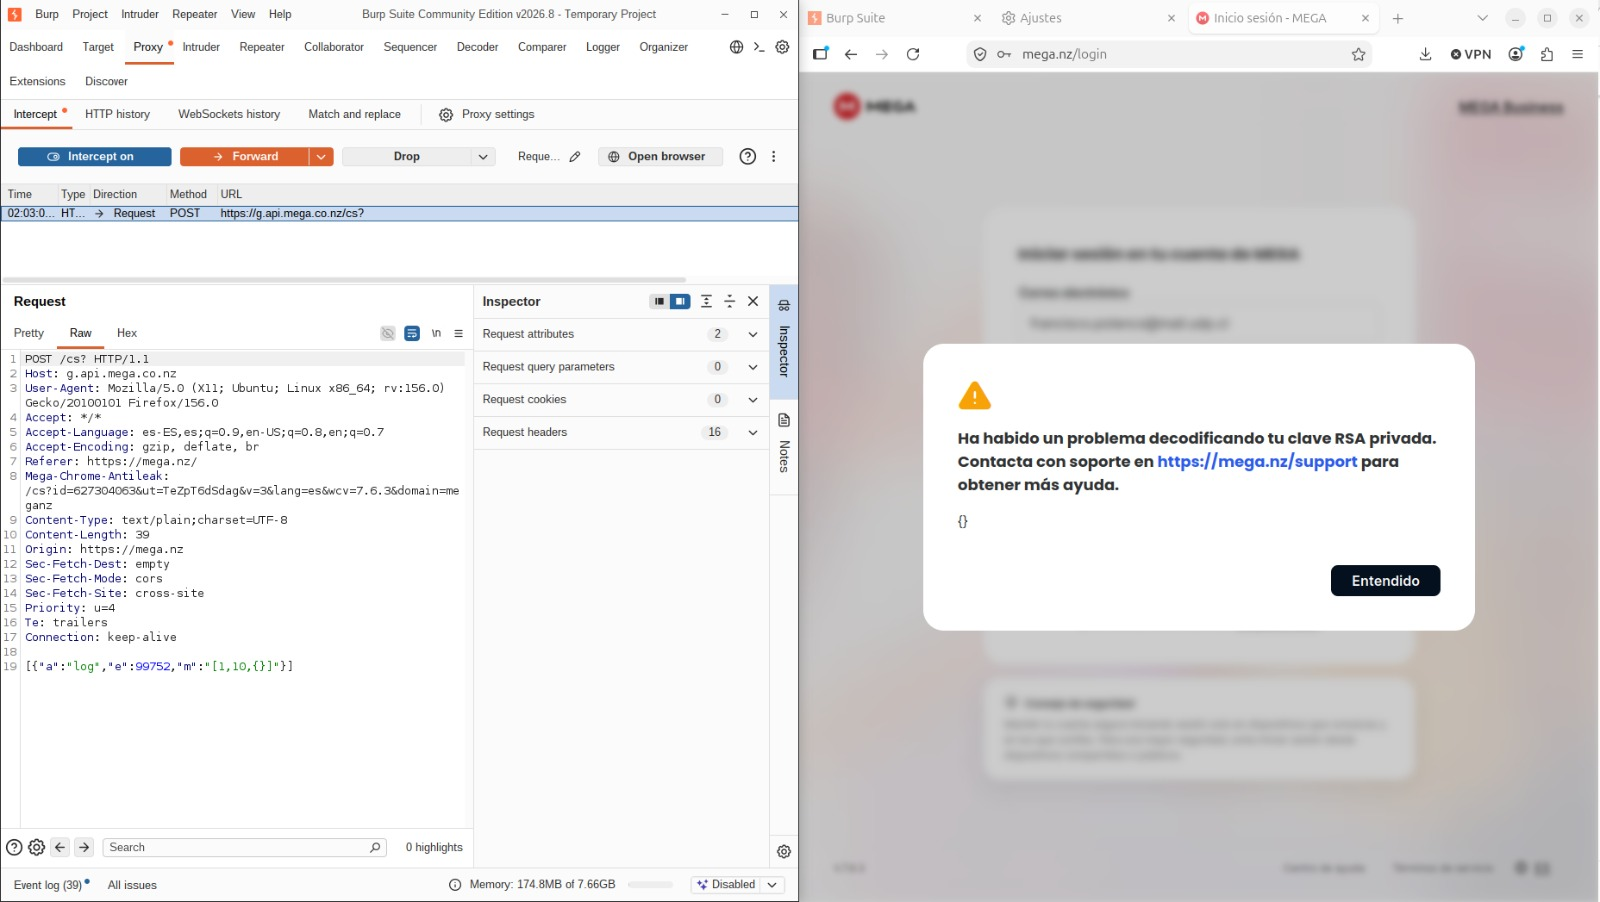
\includegraphics[width=0.95\textwidth]{fig15_pth_error_rsa.jpeg}
    \caption{Error mostrado por el cliente de Mega tras el ataque}
    \label{fig:pth-error}
\end{figure}

El mensaje mostrado por la interfaz fue \textit{``Ha habido un problema decodificando tu clave RSA privada''}. Esto ocurre porque, si bien el \texttt{uh} coincide con el valor esperado por el servidor, la password key (los primeros 16 bytes de la clave derivada por PBKDF2, usados para descifrar \texttt{k} y \texttt{privk}) fue calculada por el navegador a partir de la contraseña \textit{incorrecta} ingresada en el formulario, y por lo tanto no coincide con la clave real necesaria para descifrar la \textit{master key} y la clave privada RSA del usuario.

\subsection{Identifica las políticas de privacidad o seguridad}

\sangria Adicional a las actividades realizadas, se consultaron los documentos oficiales de Mega relacionados con el tratamiento de credenciales, la recuperación de cuentas y la protección de información cifrada, para contrastar lo observado durante el registro y la autenticación con las responsabilidades y limitaciones comunicadas por Mega. Los documentos considerados fueron:

\begin{itemize}
    \item \textbf{Política de Privacidad}: \url{https://mega.io/privacy}
    \item \textbf{Términos de Servicio}: \url{https://mega.io/terms}
\end{itemize}

Entre los puntos más relevantes relacionados con la seguridad de las contraseñas, se destacan:

\begin{itemize}
    \item La Política de Privacidad advierte explícitamente que, si el usuario olvida su contraseña, perderá el acceso a la totalidad de sus datos, a menos que haya exportado y conservado previamente una \textbf{Recovery Key}. La propia interfaz de Mega declara allí que \textit{``MEGA utiliza un cifrado de conocimiento cero para mantener la privacidad de tus datos, ni siquiera nosotros podemos acceder a tu contraseña''}, y que la Recovery Key \textit{``es la única forma de restablecer la contraseña si la olvidas''}.

    \item Esta medida es consecuencia directa de la arquitectura de cifrado de conocimiento cero que utiliza Mega: dado que la contraseña actúa como la clave de cifrado y nunca es conocida por los servidores de la empresa, Mega no tiene forma de restablecerla ni de recuperar el acceso a la cuenta si tanto la contraseña como la Recovery Key se pierden.

    \item Esto es completamente coherente con la evidencia recopilada durante este laboratorio: en ningún momento del proceso de registro o inicio de sesión la contraseña en texto plano fue transmitida al servidor; únicamente se envió el valor derivado \texttt{uh}, calculado localmente mediante PBKDF2-HMAC-SHA512.
\end{itemize}

\subsection{Demuestra 4 conclusiones sobre la seguridad}

\begin{enumerate}

    \item \textbf{Mega no utiliza un hash simple de contraseña:} A diferencia de implementaciones poco robustas que almacenan directamente una contraseña mediante, por ejemplo, \texttt{MD5(contraseña)} o \texttt{SHA256(contraseña)}, Mega deriva la contraseña mediante PBKDF2-HMAC-SHA512 con 100.000 iteraciones de cifrado y un salt único por usuario. Esto incrementa significativamente el costo computacional de un ataque de fuerza bruta o de diccionario, ya que cada intento de contraseña requiere repetir 100.000 rondas de HMAC-SHA512, y el salt único impide el uso de rainbow tables precomputadas entre distintas cuentas. Esto representa una buena práctica de seguridad frente a sitios que aún usan hashes rápidos sin mecanismos de seguridad.

    \item \textbf{La arquitectura separa la autenticación de servidor del cifrado de datos del cliente:} Se demostró experimentalmente que es posible autenticarse ante el servidor de Mega (obteniendo un \texttt{csid} válido) utilizando únicamente el valor derivado \texttt{uh}, sin necesidad de conocer la contraseña real. Sin embargo, esto por sí solo no permite acceder al contenido del usuario, ya que la \textit{master key} y la clave privada RSA solo pueden descifrarse con la \textit{password key}, la cual depende directamente de la contraseña en texto plano. Esta separación constituye una defensa en profundidad, por lo que filtrar el valor de autenticación no significa comprometer la confidencialidad de los datos almacenados.


    \item \textbf{El uso de HTTPS y de un modelo \textit{zero-knowledge} reduce el riesgo de ataque pero no lo elimina:} Todo el proceso de derivación de claves ocurre en JavaScript, ejecutado dentro del navegador del usuario. Esto significa que la seguridad de todo el esquema depende críticamente de la integridad del código servido por Mega y del entorno del navegador: un atacante capaz de inyectar código malicioso en el cliente podría capturar la contraseña en texto plano antes de que esta sea derivada, anulando por completo las protecciones criptográficas utilizadas. 

    \item \textbf{El valor \texttt{uh} funciona como una credencial equivalente a la contraseña frente al servidor:} La prueba de la Sección~\ref{sec:pth} mostró que el servidor aceptó un \texttt{uh} reemplazado manualmente y entregó un \texttt{csid} válido, sin poder distinguir si ese valor provenía de la contraseña escrita en el formulario. En la práctica, quien obtenga el \texttt{uh} (por ejemplo, desde tráfico interceptado en un equipo comprometido o con un certificado raíz malicioso instalado, como el de BurpSuite en este laboratorio) puede autenticarse sin conocer la contraseña, ya que el mismo valor fue aceptado en un inicio de sesión distinto al original. Esto se mitiga con la autenticación en dos factores y con el hecho de que los datos siguen cifrados con la \textit{password key}, pero evidencia que proteger el \texttt{uh} es tan importante como proteger la contraseña.

\end{enumerate}


\end{document}